\documentclass[12pt]{article}
\usepackage{hyperref}
\usepackage{amsmath}
%\usepackage{amsmath}
\usepackage{graphicx}
% \usepackage[extendedchars]{grffile}
\usepackage{chngpage}
\usepackage{calc}


\title{Generation SM particles that subsequently decay into millicharged particles}

\author{C. Campagnari (UCSB), F. Golf (UNL), B. Marsh (UCSB)}

\begin{document}
\maketitle


\section{Introduction}
In this document we discuss the generation of SM particles that in 
a subsequent step will be made to decay into milliCharged particles.
The key features of our approach are the following
\begin{itemize}
\item Use theory or published data, or some MC to generate $P_T$ distributions for SM
  particles
saved as histograms in ROOT files (Drell Yan is an exception, see
discussion in Section~\ref{sec:DY}).
\item Sample the ROOT histograms to generate SM particles of a 
given $P_T$
\item Pick azimuthal angles $\phi$ and pseudorapity $\eta$ in a
  limited 
range, matched to the acceptance of milliqan.
\item Decay the SM particles into milliCharged particles (this 
step is described in a separate note).  
\item When possible, keep track of theoretical uncertainties.
\item In general it is sufficient to generate SM particles at low 
and moderate $P_T$ since that is where the cross-section is largest.
\end{itemize}

\section{Drell Yan}
\label{sec:DY}

Golf needs to fix his bugs.

\section{J/$\psi$ and $\psi'$ from b-decays}
\label{sec:bpsi}
We use the tool available in \\
\href{http://www.lpthe.jussieu.fr/~cacciari/fonll/fonllform.html}
{http://www.lpthe.jussieu.fr/~cacciari/fonll/fonllform.html} \\
to
generate histograms of $P_T$ distributions (cross-sections) for charmonium from 
bottom decays, including theoretical 
uncertainties\cite{Cacciari:2012ny,Cacciari:2015fta}.  
See Figure~\ref{fig:bpsi} 

\begin{figure}
  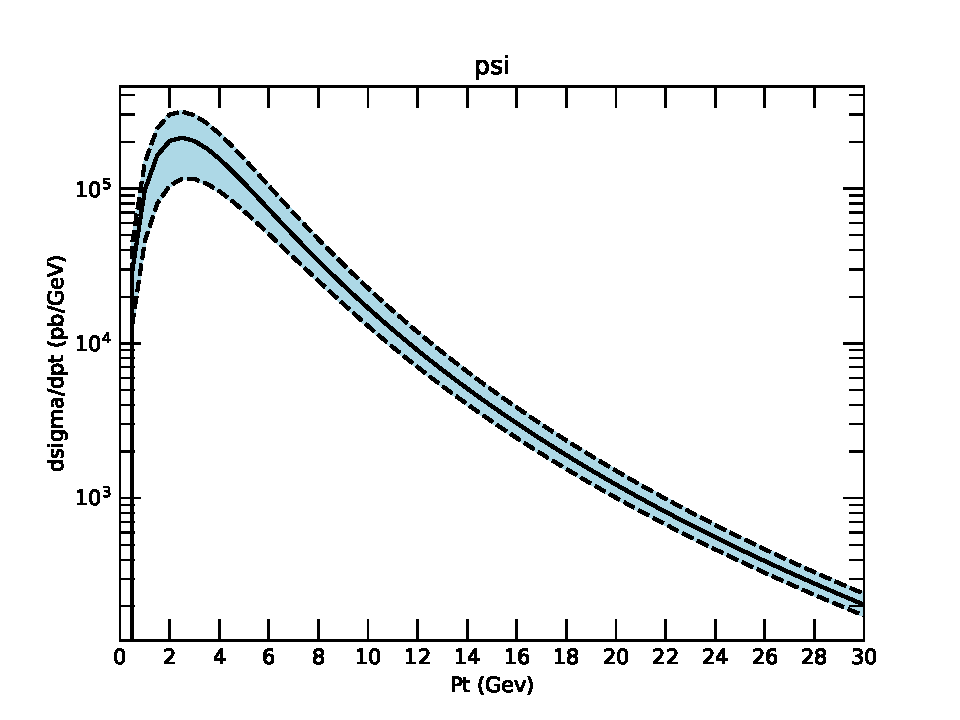
\includegraphics[width=0.48\linewidth]{../oniaFromB/psi.pdf}
  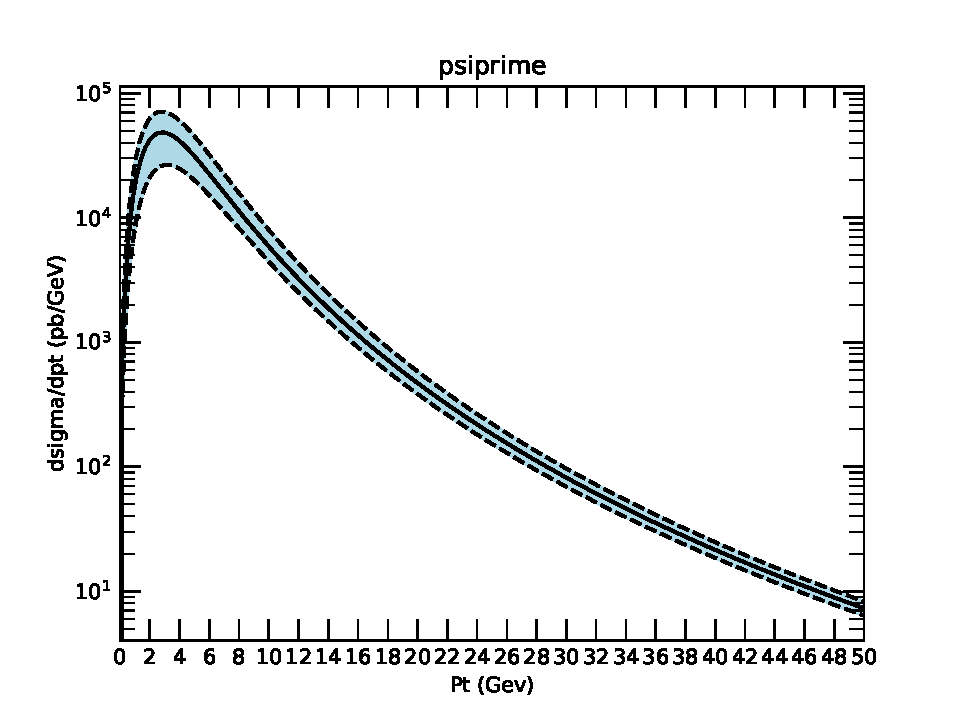
\includegraphics[width=0.48\linewidth]{../oniaFromB/psiprime.pdf}
  \caption{Transverse momentum distributions of J/$\psi$ (left) 
and $\psi'$ from bottom quark decays. Note: this is from a single $b$, 
multiply by two to include $\bar{b}$.}
  \label{fig:bpsi}
\end{figure}

\section{Direct onia production}
\label{sec:onia}

\subsection{Direct bottonium}
\label{sec:upsilon}

There have been many measurement of the $P_T$ spectra od $\Upsilon$ in $pp$ collisions
at the LHC by CMS~\cite{Khachatryan:2010zg, Chatrchyan:2013yna, Khachatryan:2015qpa, Sirunyan:2017qdw},
Atlas~\cite{Aad:2011xv, Aad:2012dlq},
  and LHCb~\cite{Aaij:2018pfp, Aaij:2015awa, Aaij:2014nwa, Aaij:2013yaa, LHCb:2012aa}.
  The LHCb measurements are in the forward region.  The only measurement at 13 TeV
  in the central region is from CMS~\cite{Sirunyan:2017qdw}.  Unfortunately, it is limited
  to $P_T >$ 20 GeV.

  Due to the lack of 13 TeV data, initially we planned to use theoretical predictions
  as a basis of the $\Upsilon$ event generation.
  We contacted the theorists~\cite{Han:2014kxa}
  that provided the state-of-the art calculations used to
  confront the data in Reference~\cite{Sirunyan:2017qdw}.  We
  asked them to extend their predictions to lower $P_T$, unfortunately they claim that these
  are unreliable below 15 GeV.

\begin{figure}
\begin{adjustwidth}{-3cm}{-3cm}
\centering
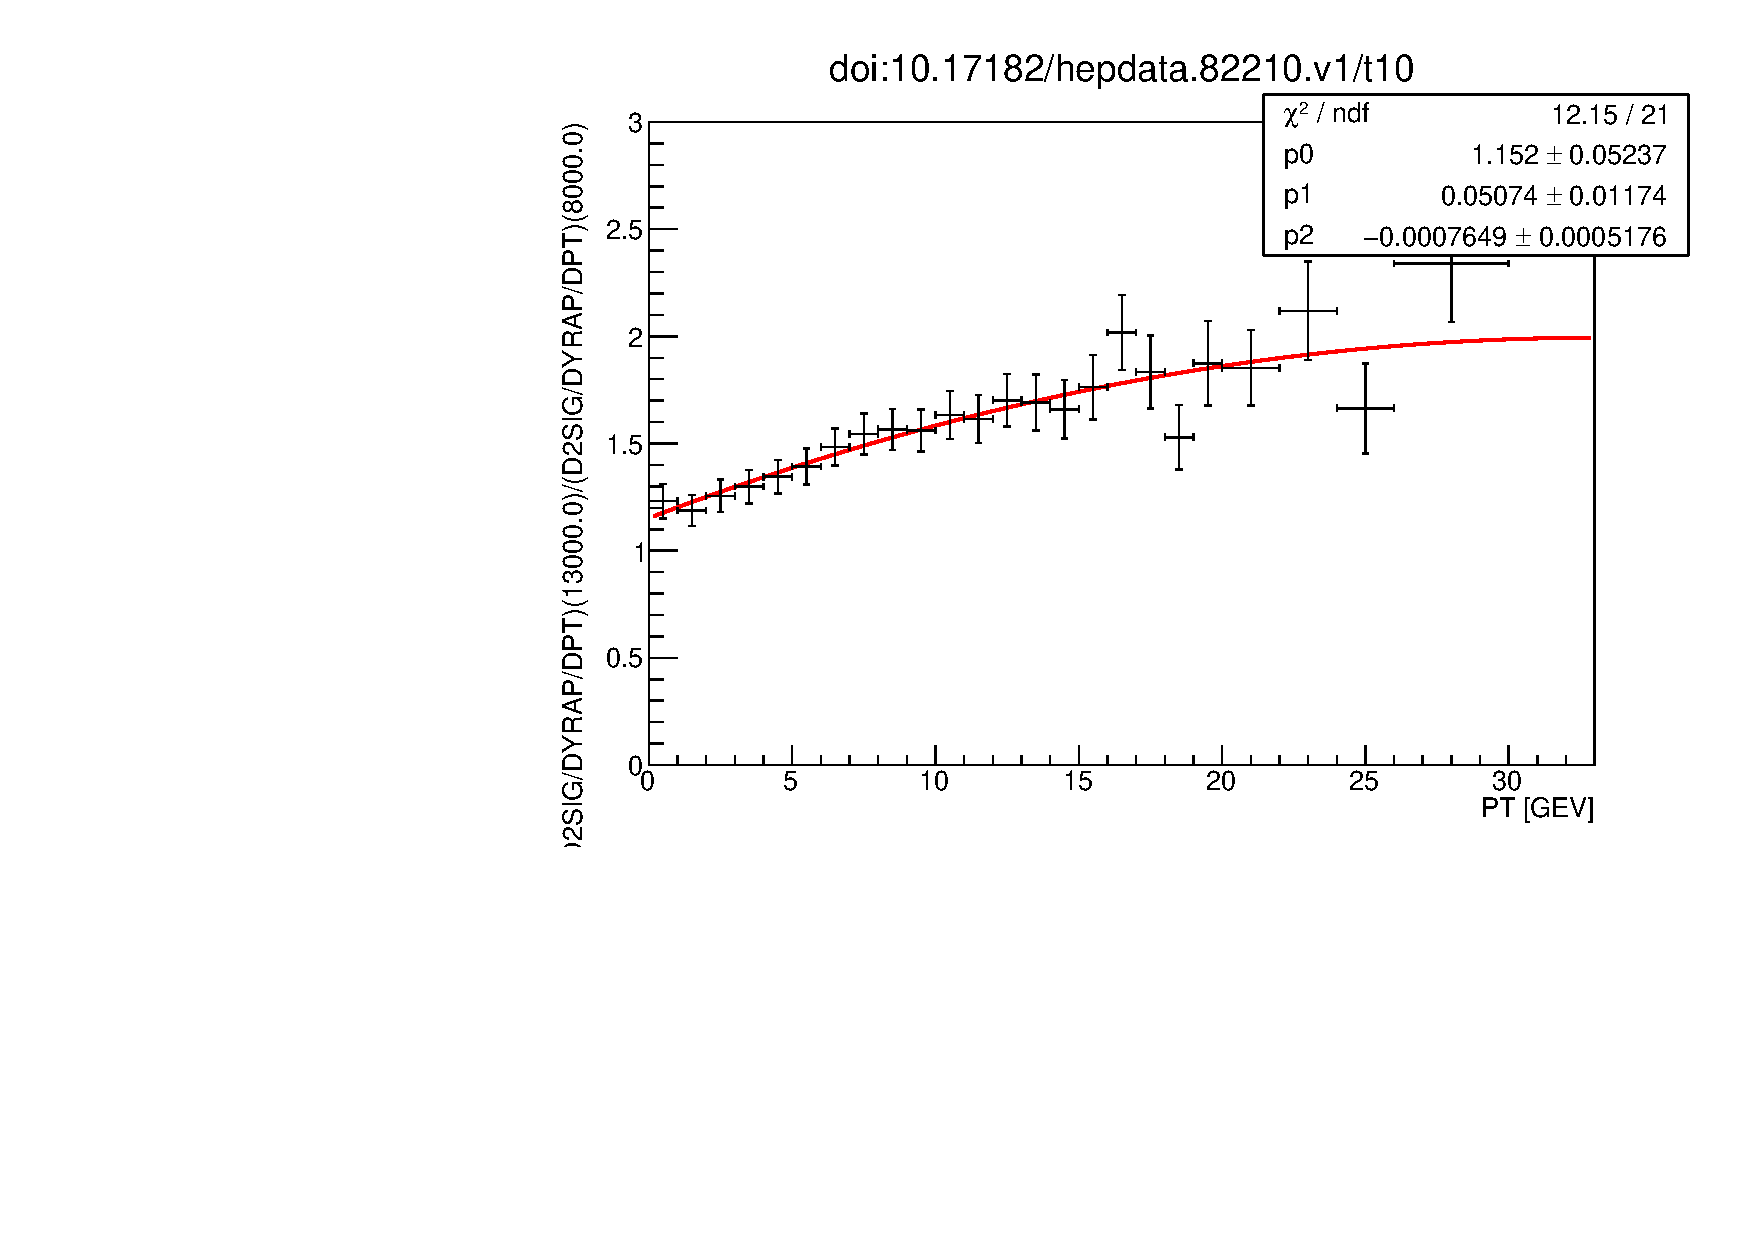
\includegraphics[width=0.32\linewidth]{../oniaDirect/LHCB-13-TeV/ups1s-13to7eta20to25.pdf}
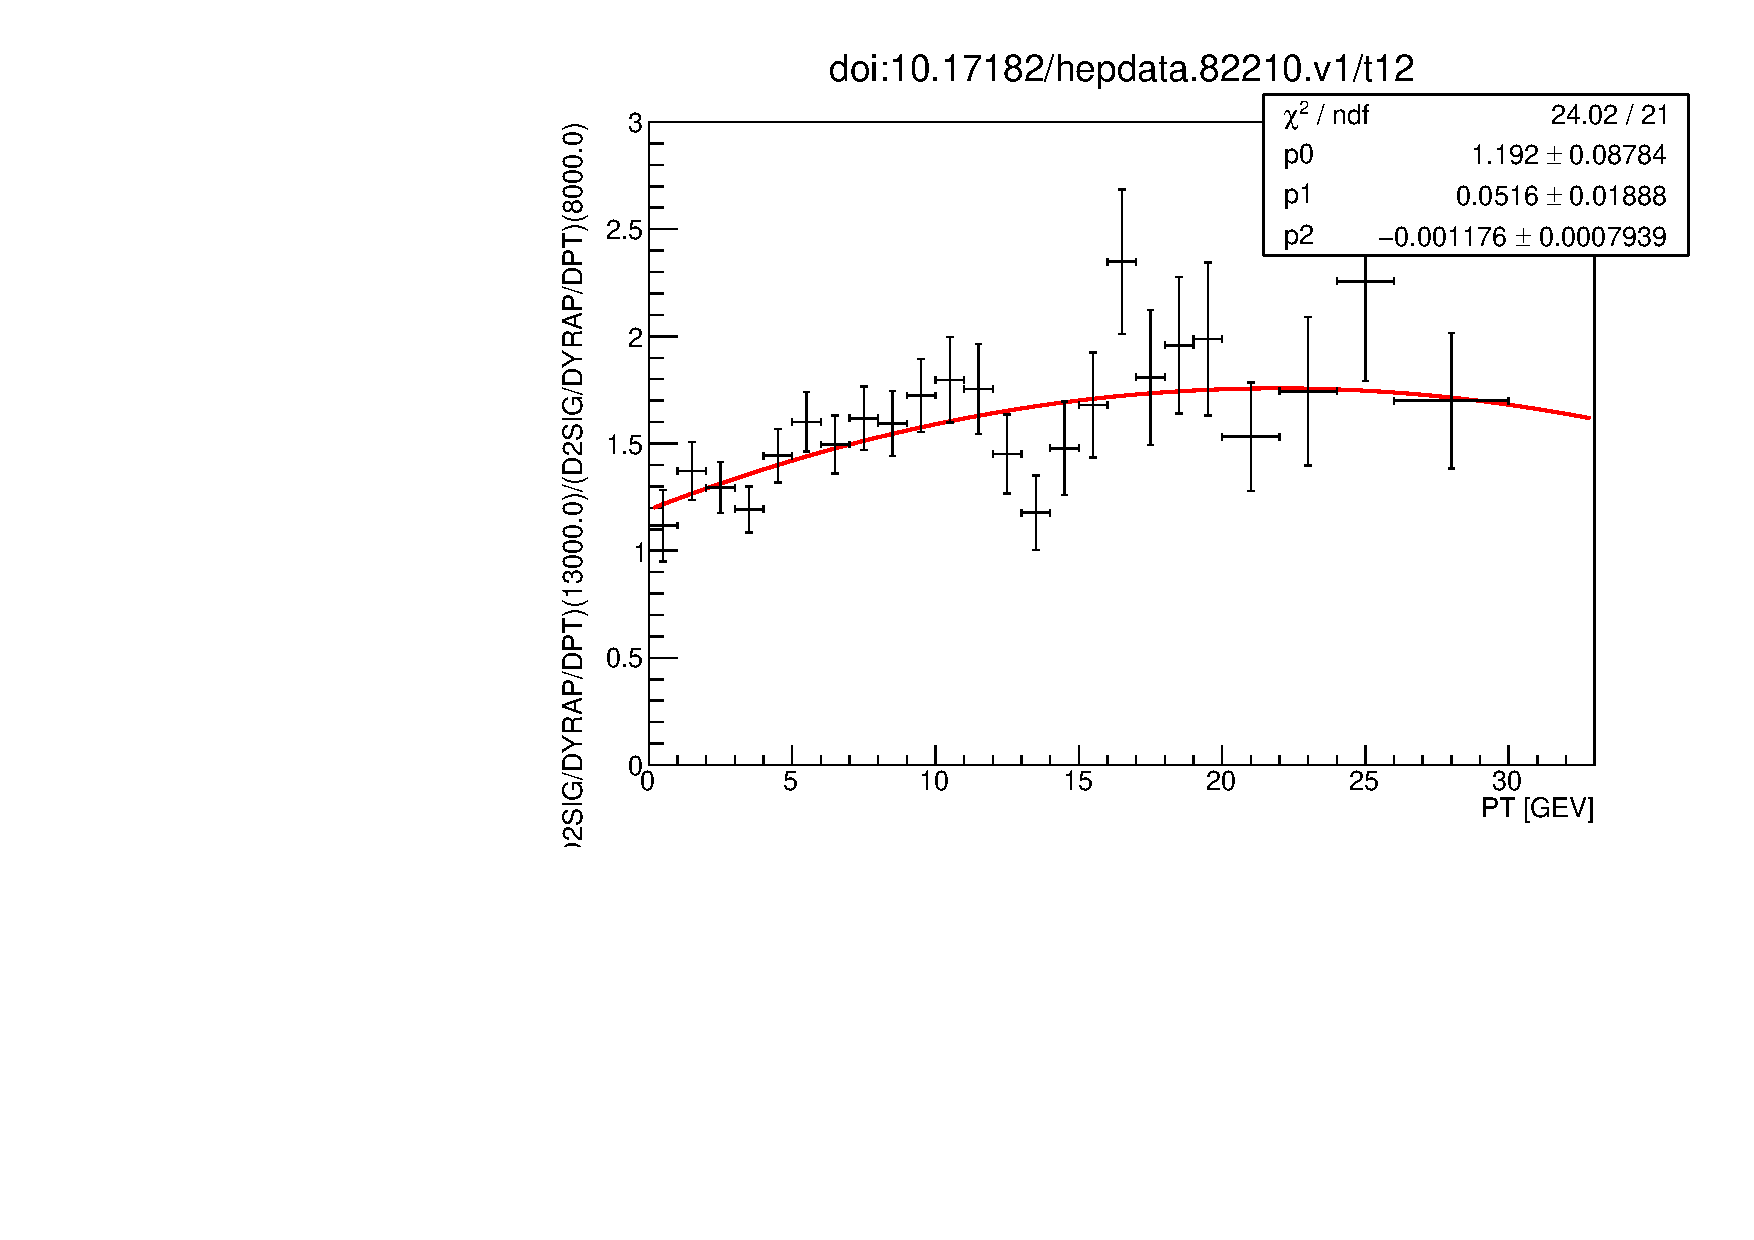
\includegraphics[width=0.32\linewidth]{../oniaDirect/LHCB-13-TeV/ups3s-13to7eta20to25.pdf}
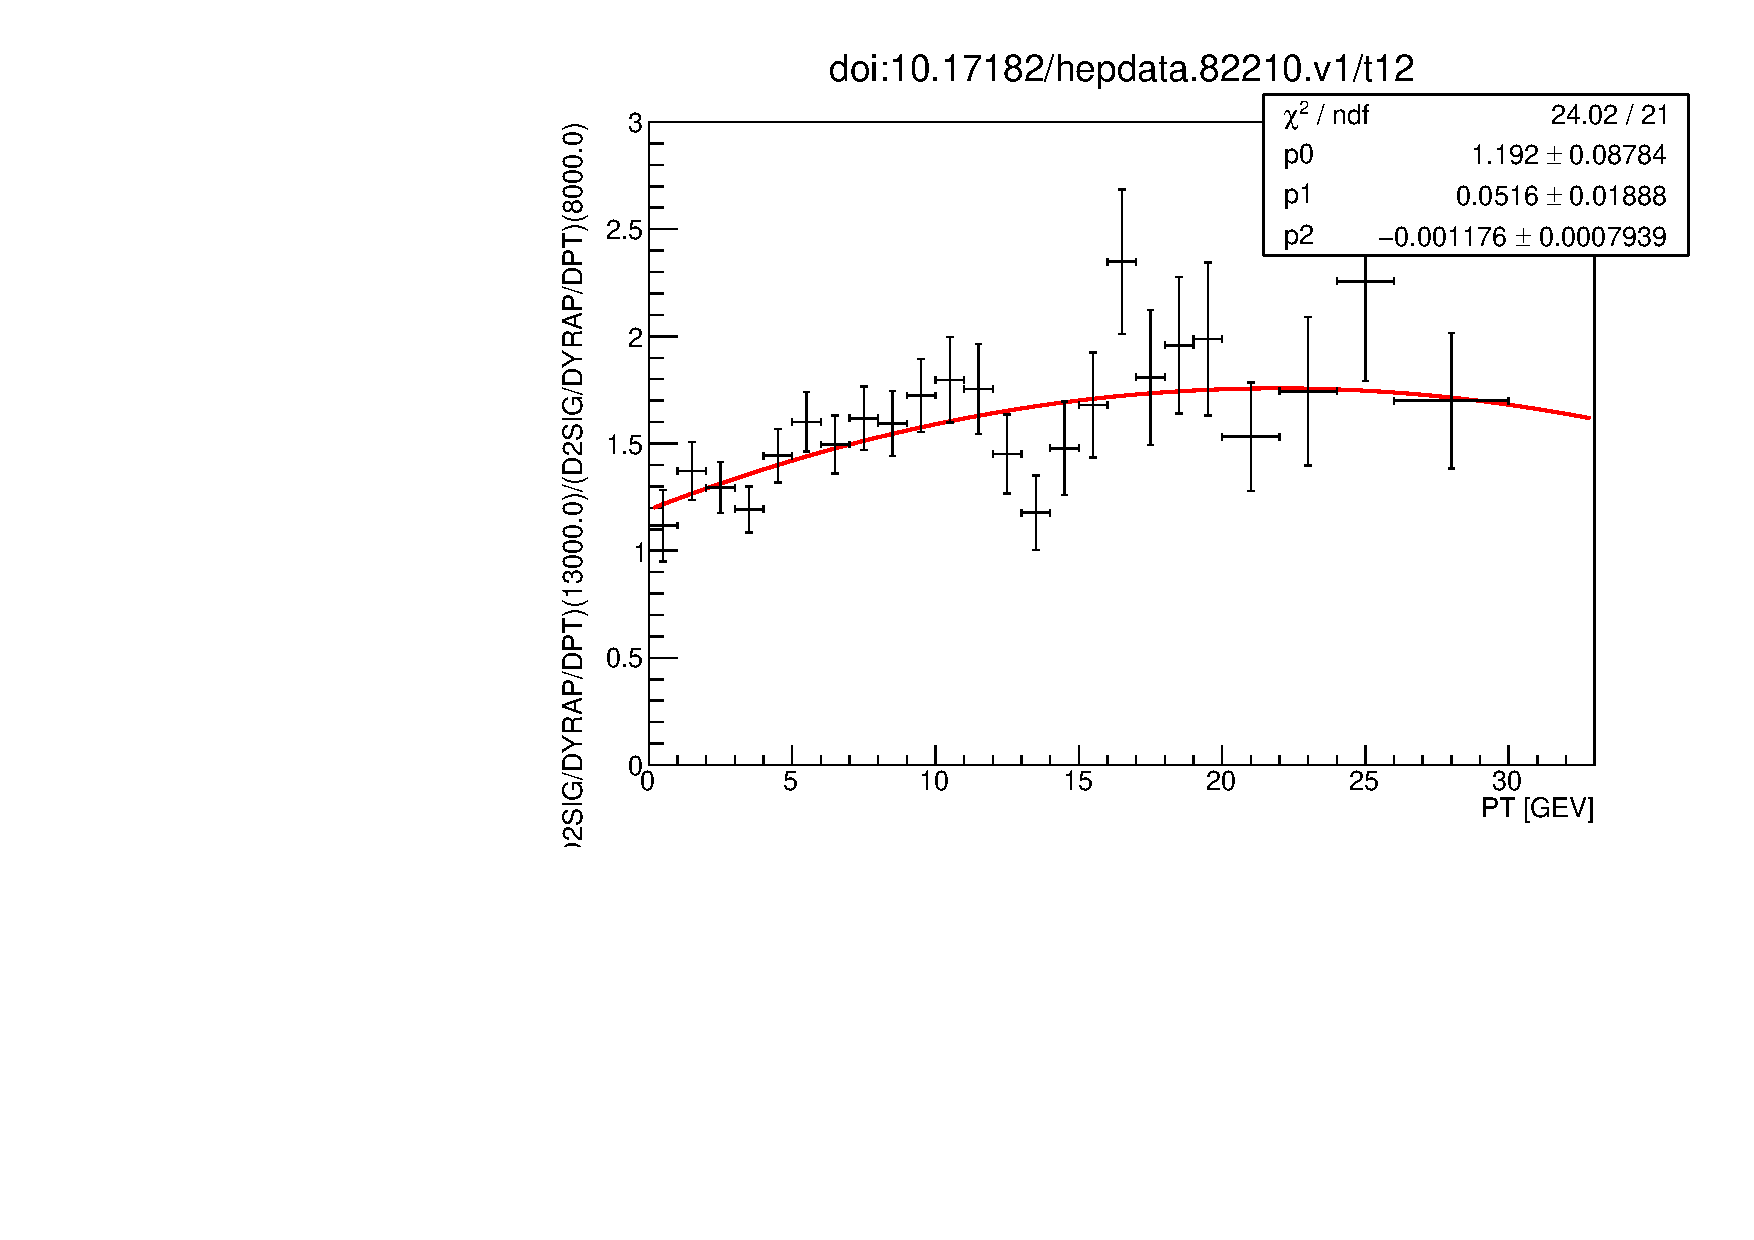
\includegraphics[width=0.32\linewidth]{../oniaDirect/LHCB-13-TeV/ups3s-13to7eta20to25.pdf}
\end{adjustwidth}
\caption{\protect Ratio of 13 to 7 GeV $\Upsilon$ cross-section for $2.0 < |\eta| < 2.5$
  from LHCb~\cite{Aaij:2018pfp}.  From left to right: 1S, 2S, 3S. 
  The quadratic fits are ours.}
\label{fig:upsratio}
\end{figure}

  
  As a result we decided to use 7 TeV data for $P_T <$ 20 GeV and the CMS
  13 TeV data at higher $P_T$.  A key ingredient is the ratio of 13 and 7
  GeV $\Upsilon$ production cross-sections.  These have been measured
  for $P_T > 20$ GeV and $|\eta| <$ 1.2 by CMS,
  see Figure 2 of Reference~\cite{Sirunyan:2017qdw}. The ratios
  are about 1.7 at $P_T$ = 20 GeV, irrespective of $\Upsilon$ state
  (1S, 2S, or 3S), and increase slowly to about 2
  at $P_T$ = 40 GeV.  The ratios have also been measured by
  LHCb~\cite{Aaij:2018pfp}
  all the way down to zero $P_T$ for $2.0 < |\eta| < 2.5$, see Figure~\ref{fig:upsratio}.
  These ratios in the 20-30 GeV region are in agreement with the central
  ratios measured by CMS.

\begin{figure}
\begin{adjustwidth}{-3cm}{-3cm}
\centering
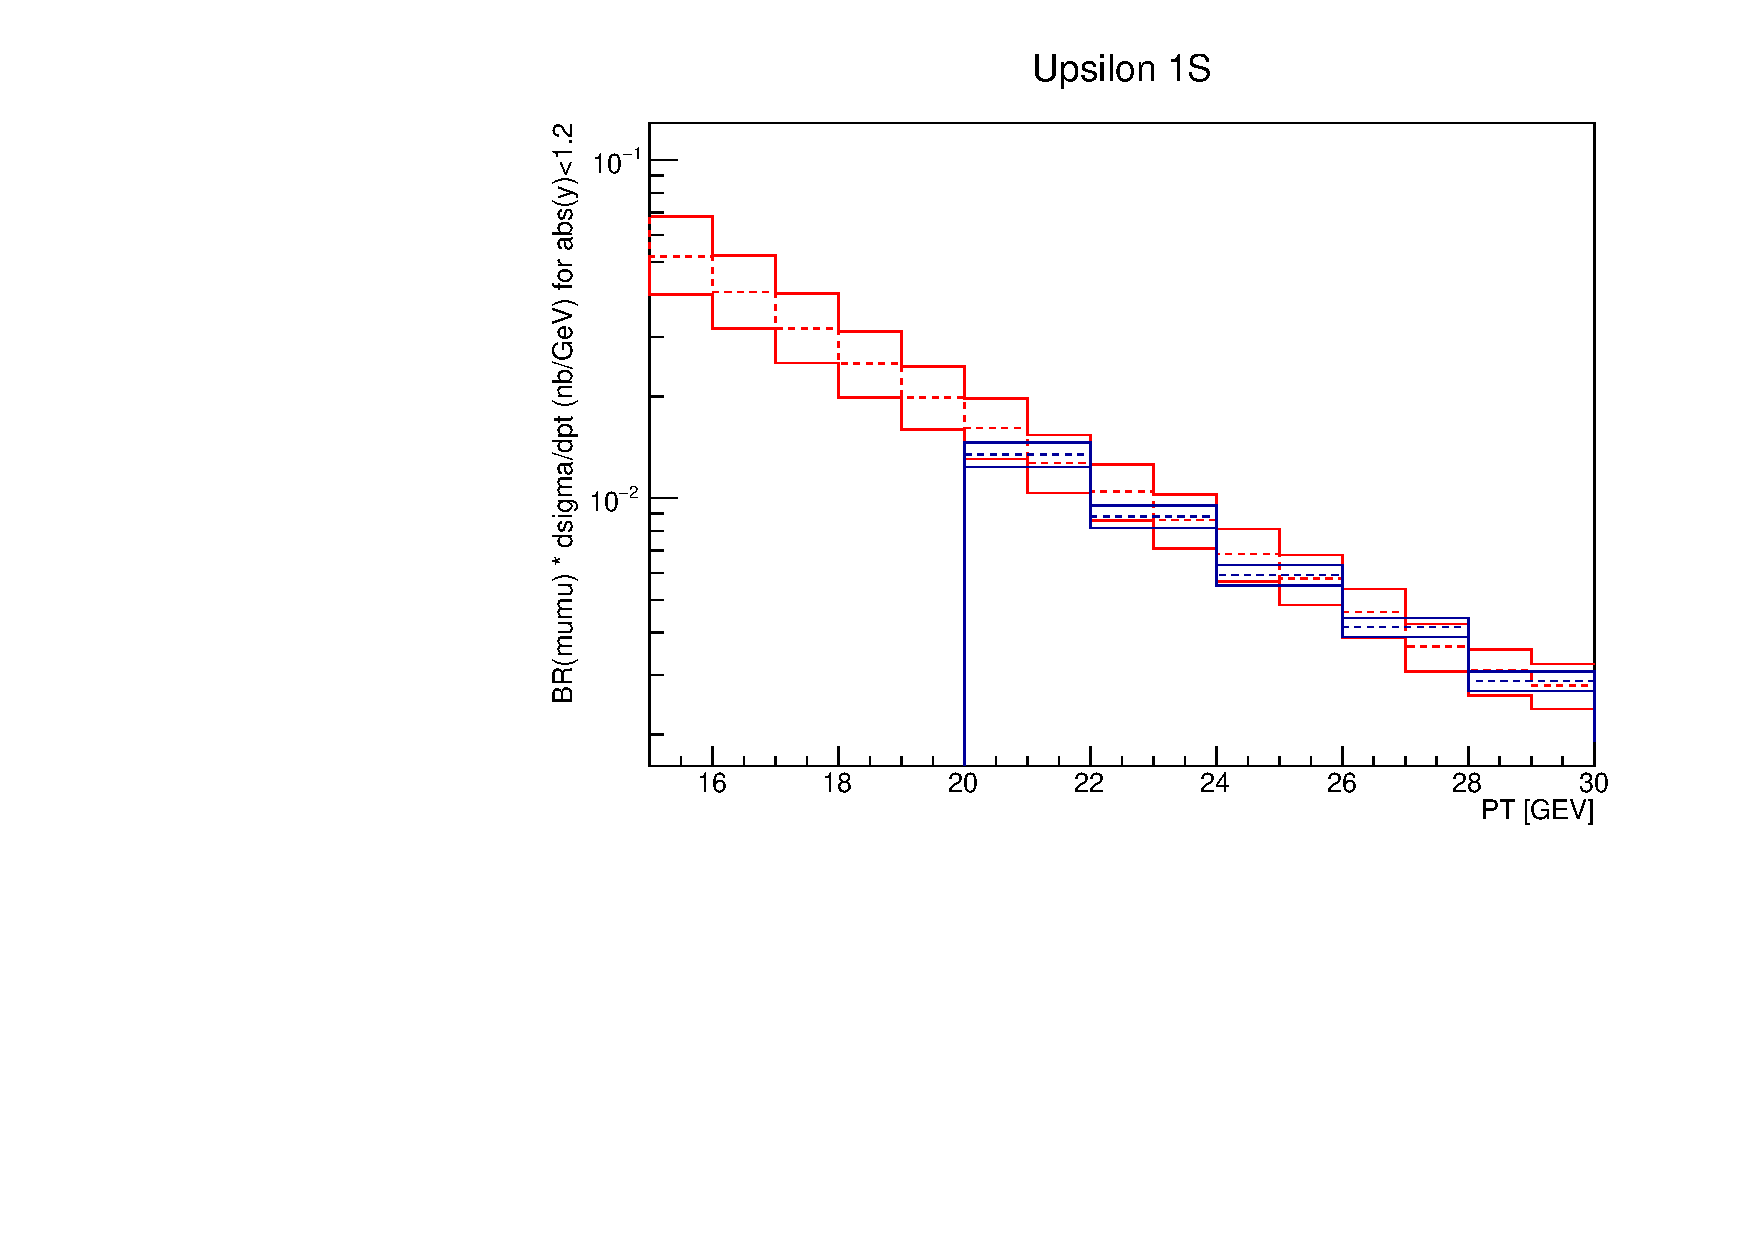
\includegraphics[width=0.32\linewidth]{../oniaDirect/upsilon/upsilon-1s-atlas-cms-comparison.pdf}
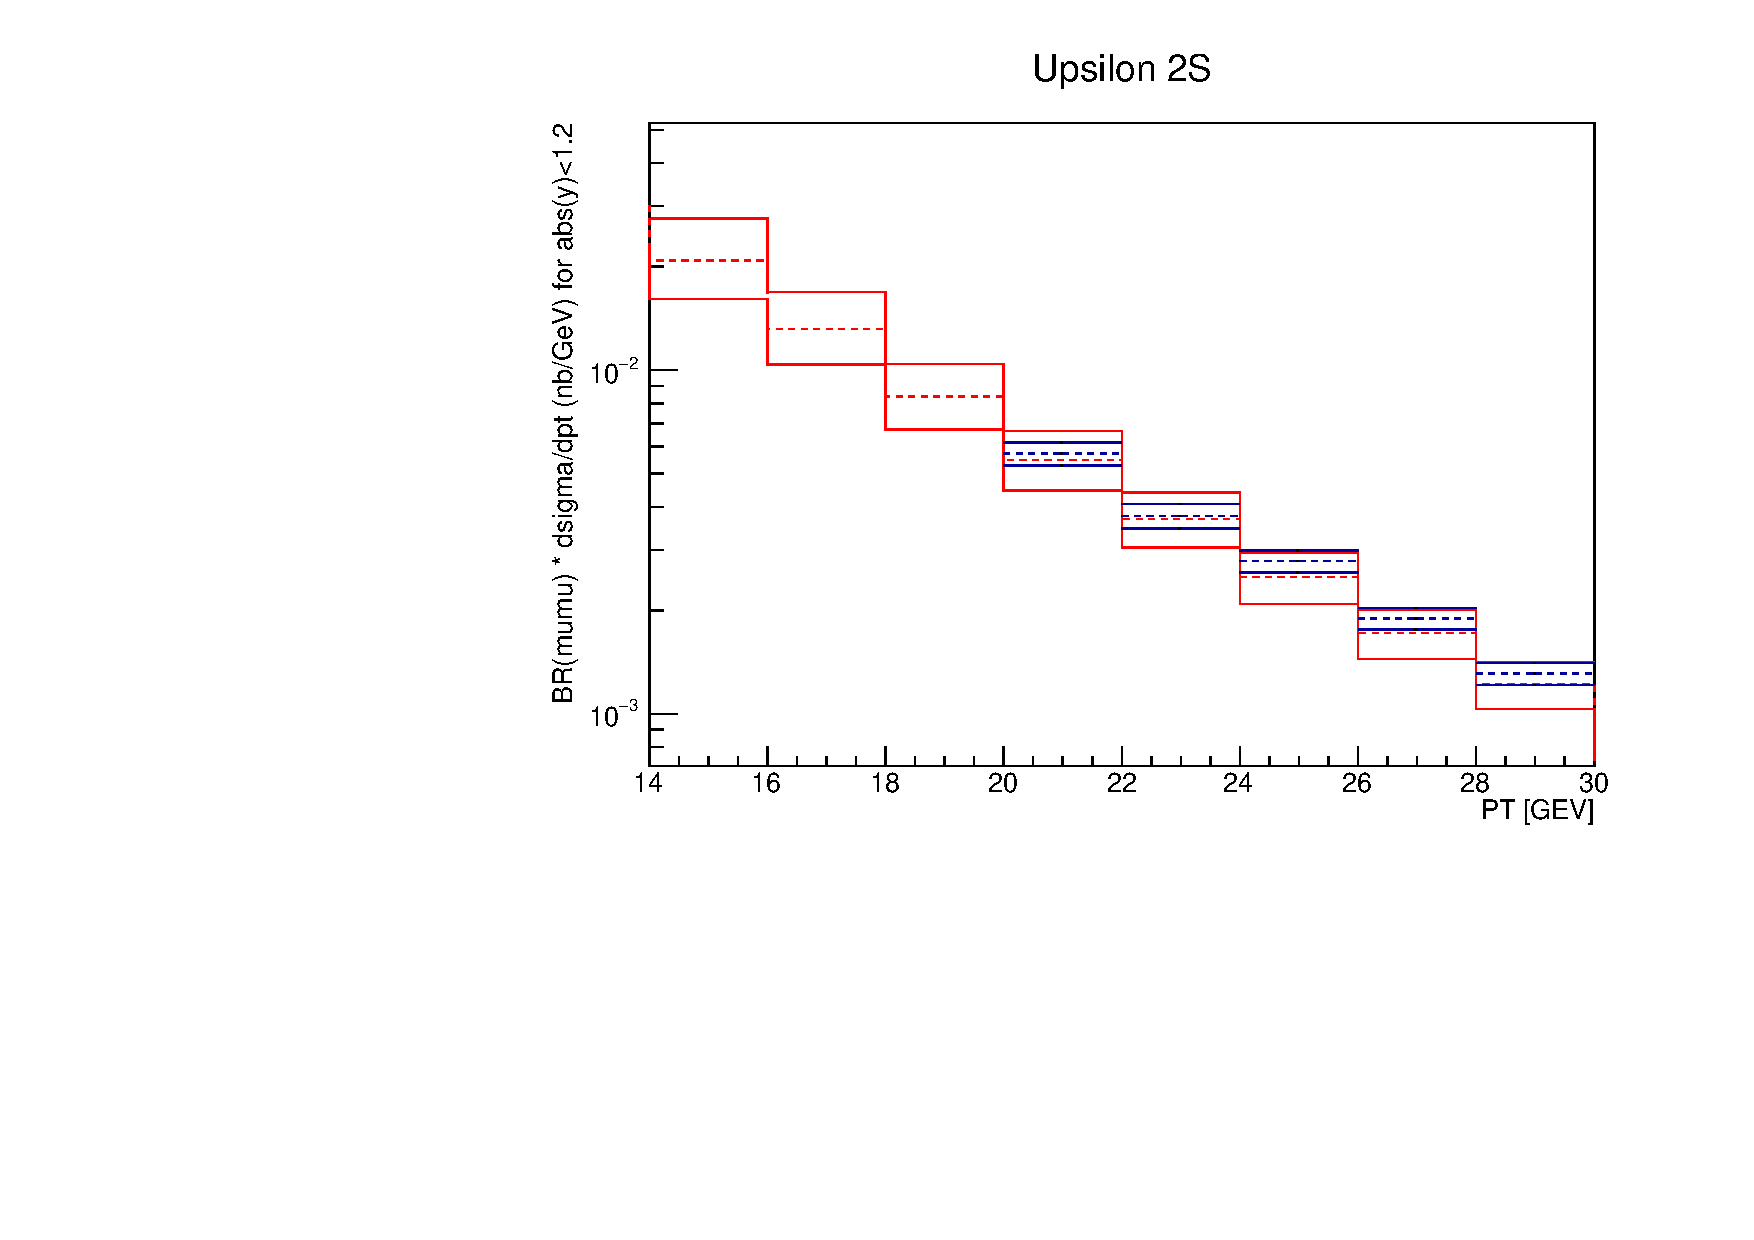
\includegraphics[width=0.32\linewidth]{../oniaDirect/upsilon/upsilon-2s-atlas-cms-comparison.pdf}
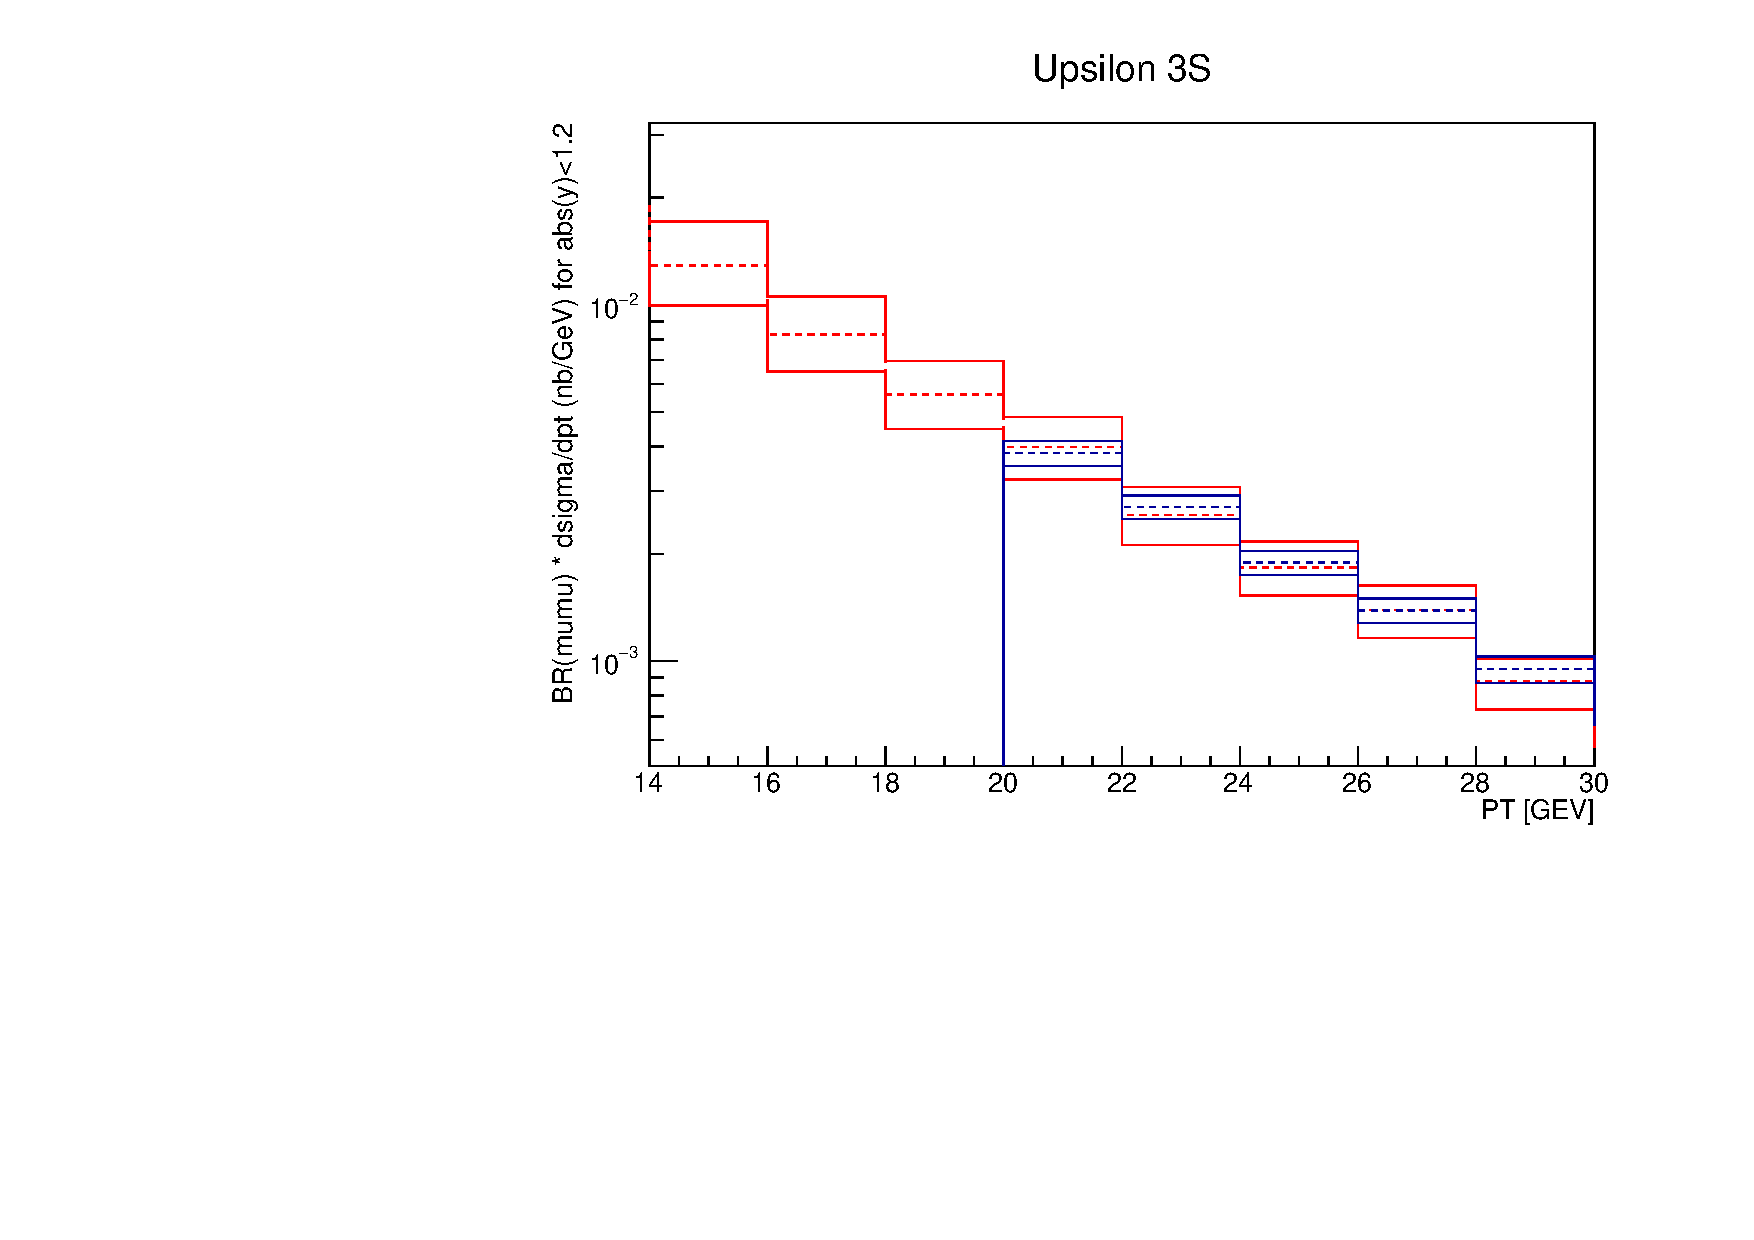
\includegraphics[width=0.32\linewidth]{../oniaDirect/upsilon/upsilon-3s-atlas-cms-comparison.pdf}
\end{adjustwidth}
\caption{\protect Comparison of the rescaled 7 GeV Atlas $\Upsilon$ spectra (red) with the
  13 GeV CMS spectra (blue) in the neighborhood of 20 GeV, where the matching of
  the two spectra takes place.  From left to right: 1S, 2S, 3S.
  The dashed lines represent the central values, the solid
  lines cover the uncertainty range.  This is ${\cal B}(\Upsilon \to \mu\mu) \cdot
  \rm{d}\sigma/\rm{d}P_T$ in nb/GeV integrated
  over $|\eta| <$ 1.2.}
\label{fig:checkMatch}
\end{figure}

\begin{figure}
\begin{adjustwidth}{-3cm}{-3cm}
\centering
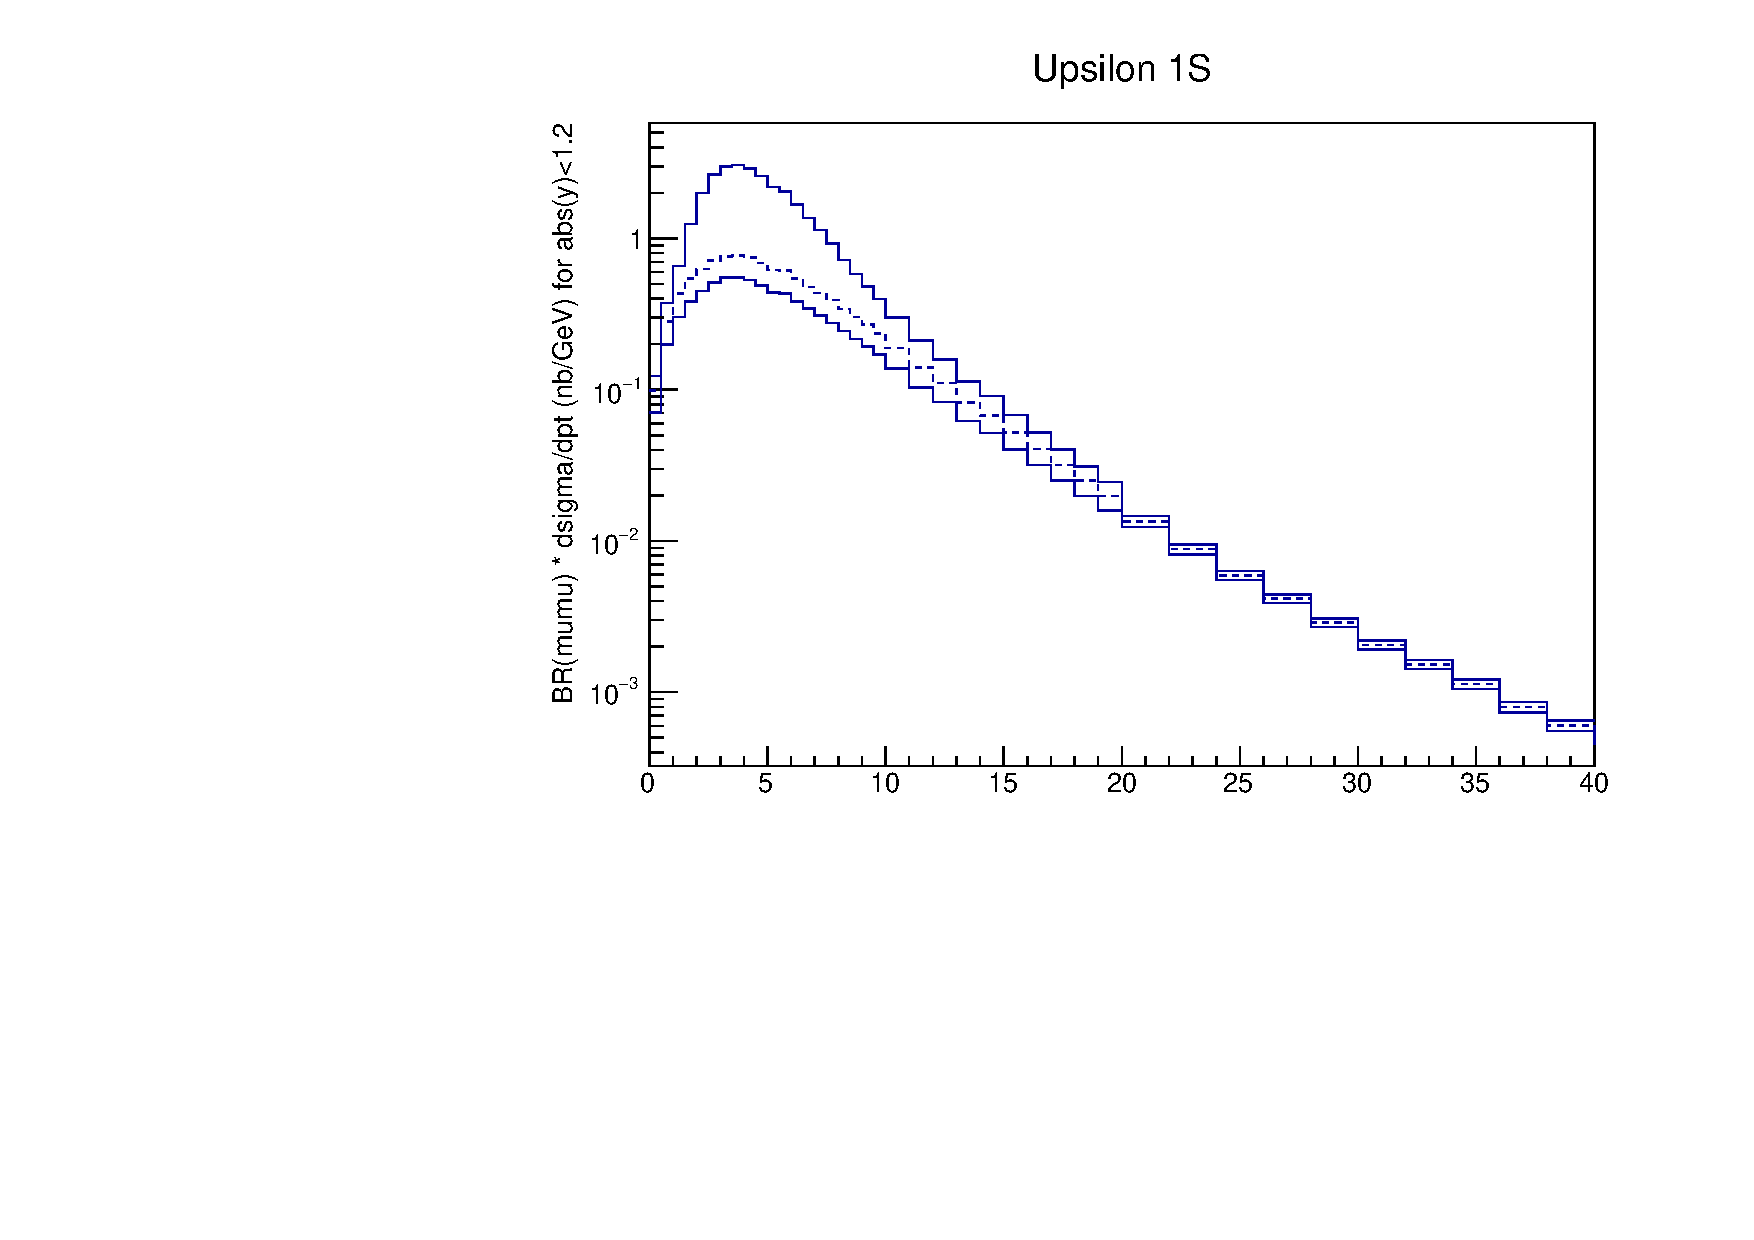
\includegraphics[width=0.32\linewidth]{../oniaDirect/upsilon/ups1s-full.pdf}
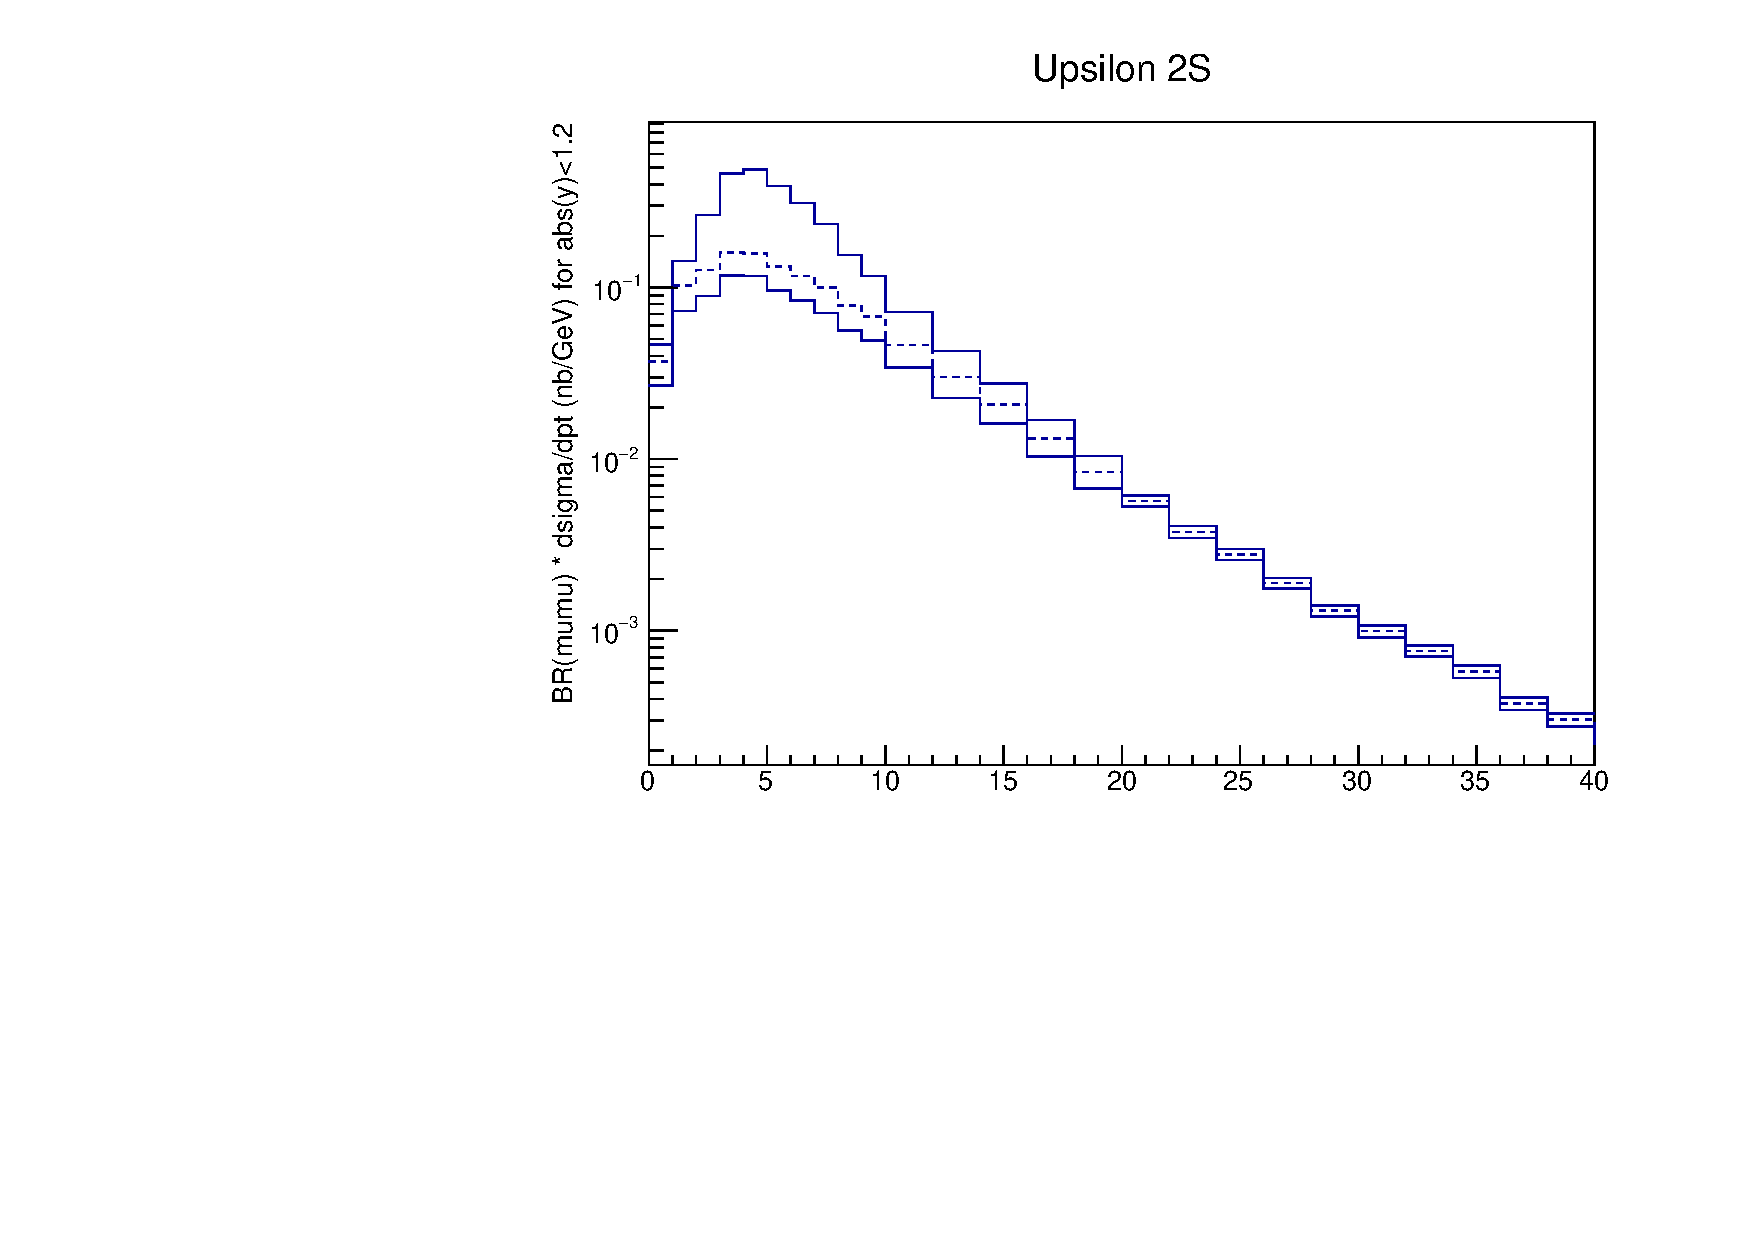
\includegraphics[width=0.32\linewidth]{../oniaDirect/upsilon/ups2s-full.pdf}
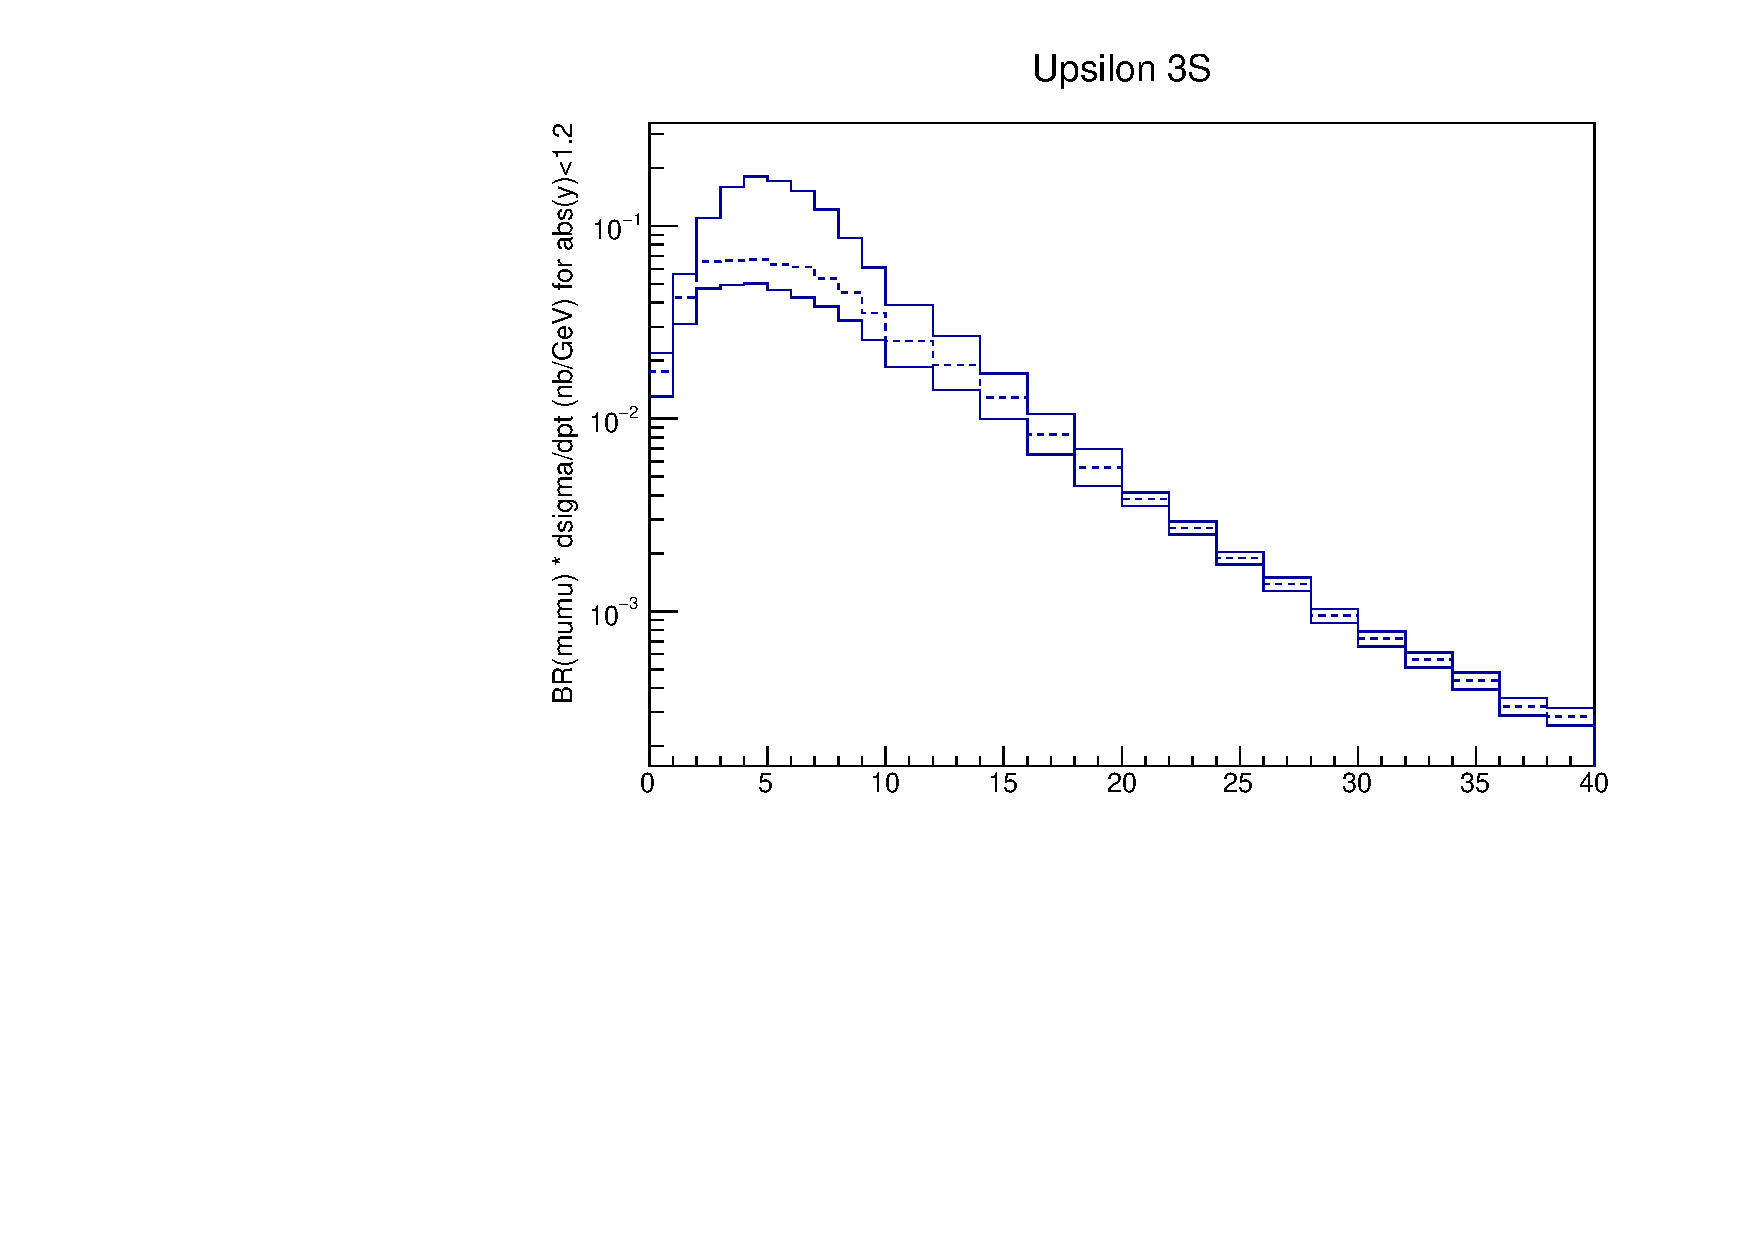
\includegraphics[width=0.32\linewidth]{../oniaDirect/upsilon/ups3s-full.pdf}
\end{adjustwidth}
\caption{\protect Combined Atlas 7 TeV, CMS 13 TeV $\Upsilon$ spectra.
  From left to right: 1S, 2S, 3S. 
The dashed line represent the central value, the solid
  lines cover the uncertainty range.  This is ${\cal B}(\Upsilon \to \mu\mu) \cdot
  \rm{d}\sigma/\rm{d}P_T$ in nb/GeV integrated
  over $|\eta| <$ 1.2.}
\label{fig:upsFinal}
\end{figure}

  
  We rescale the measured 7 GeV central low $P_T$ $\Upsilon$ spectra to 13 TeV using the
  fitted curves of Figure~\ref{fig:upsratio};  we combine these with the 13 TeV measured
  central high $P_T$ spectra to obtain an inclusive 13 TeV spectrum.  The 7 TeV data
  is from Atlas~\cite{Aad:2012dlq}, and the 13 TeV spectrum is from
  CMS~\cite{Sirunyan:2017qdw}. We demonstrate in Figure~\ref{fig:checkMatch} that the
  matching of the Atlas and CMS cross-sections works well.  The combined
  spectrum to be used in the event generation is in Figure~\ref{fig:upsFinal}.

  
  
\subsection{Direct charmonium}


\section{$\pi^0$, $\eta$, $\eta'$, $\phi$, $\rho$, and $\omega$}
\label{sec:mesons}

We generate these from Pythia.  The measurement of the 
$\pi^{\pm}$
$P_T$ spectrum from CMS\cite{Sirunyan:2017zmn} is in good agreement
with Pythia 8 Minimum Bias at low momentum.  We use this MC for all
mesons.  We do not attempt to use QCD $2 \to 2$ at very low $P_T$ since the 
process is infrared divergent.
Note that Pythia {\tt SoftQcd:nonDiffractive} includes all
hard QCD processes\cite{wwwPythia} so in principle this is all that is
needed.    However, one runs out of statistics at high $P_T$.  So 
at high $P_T$ we stitch together the minimum bias distributions with 
distributions obtained from QCD $2 \to 2$ at moderate $P_T$.

Eventually we will generate Pythia events in ``standalone'' mode to
be independent of CMS software.  For now we use existing CMS Monte
Carlos
for Minimum Bias and for QCD.  The CMS QCD samples are
``$P_T$-binned'',
(15-30 GeV, 30-50 GeV, and 50-80 GeV).  The Minimum Bias 
cross-section 
is taken to be 78.4 mb.  Then the stitching procedure is the following:
\begin{itemize}
\item The QCD samples are first normalized to their LO cross-sections.
\item next, we estimate a ``qcd-minbias scale factor'' by integrating
  over some region where the ratio is roughly flat
\item the QCD samples are renormalized by this scale factor
\item the samples are then stitched together by visually picking the 
$P_t$ where the curves cross each other.
\end{itemize}
\noindent The resulting $P_T$ curves are shown in
Figure~\ref{fig:mesons}.  It is not clear what kind of uncertainties
we should assign.  Let's first see how important these are at the end
of the day before going crazy.

\begin{figure}
  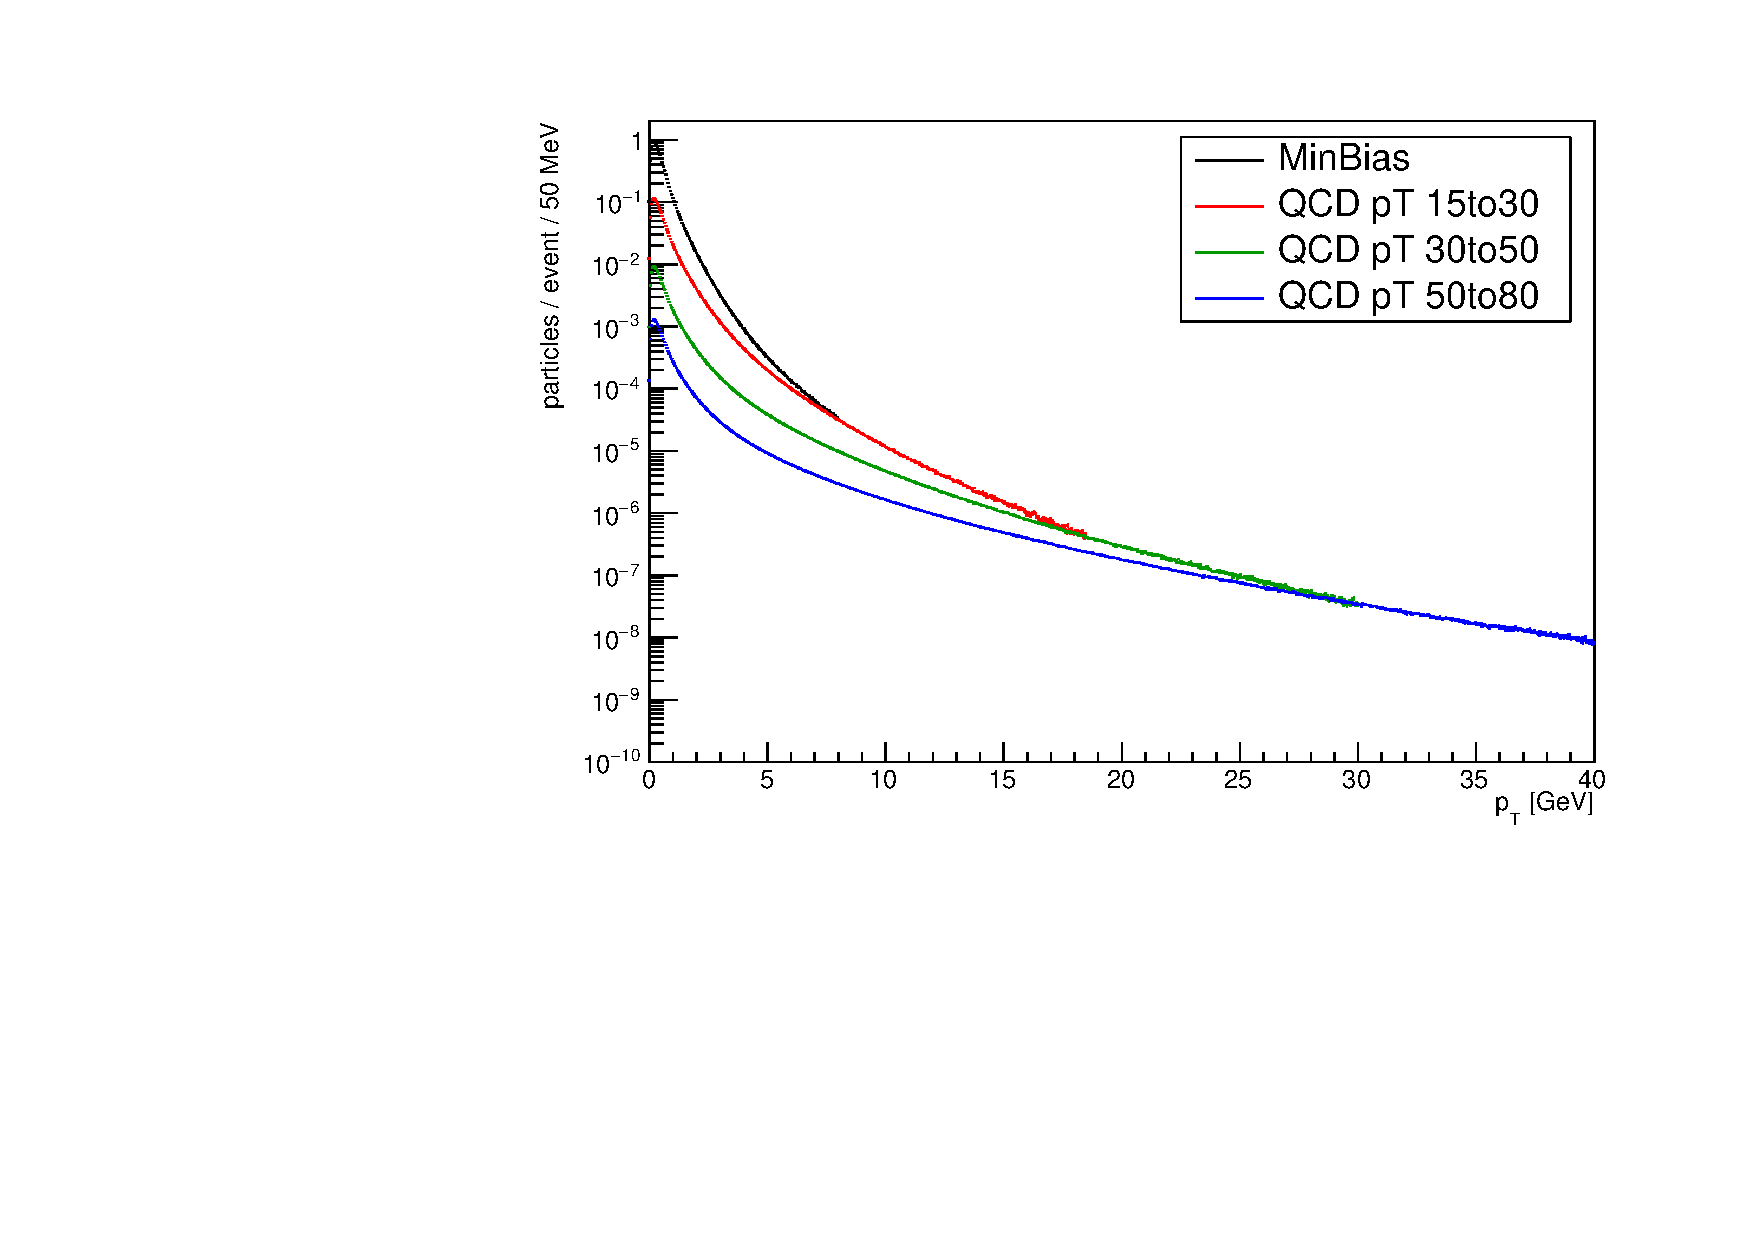
\includegraphics[width=0.48\linewidth]{plots/h_pi0.pdf}
  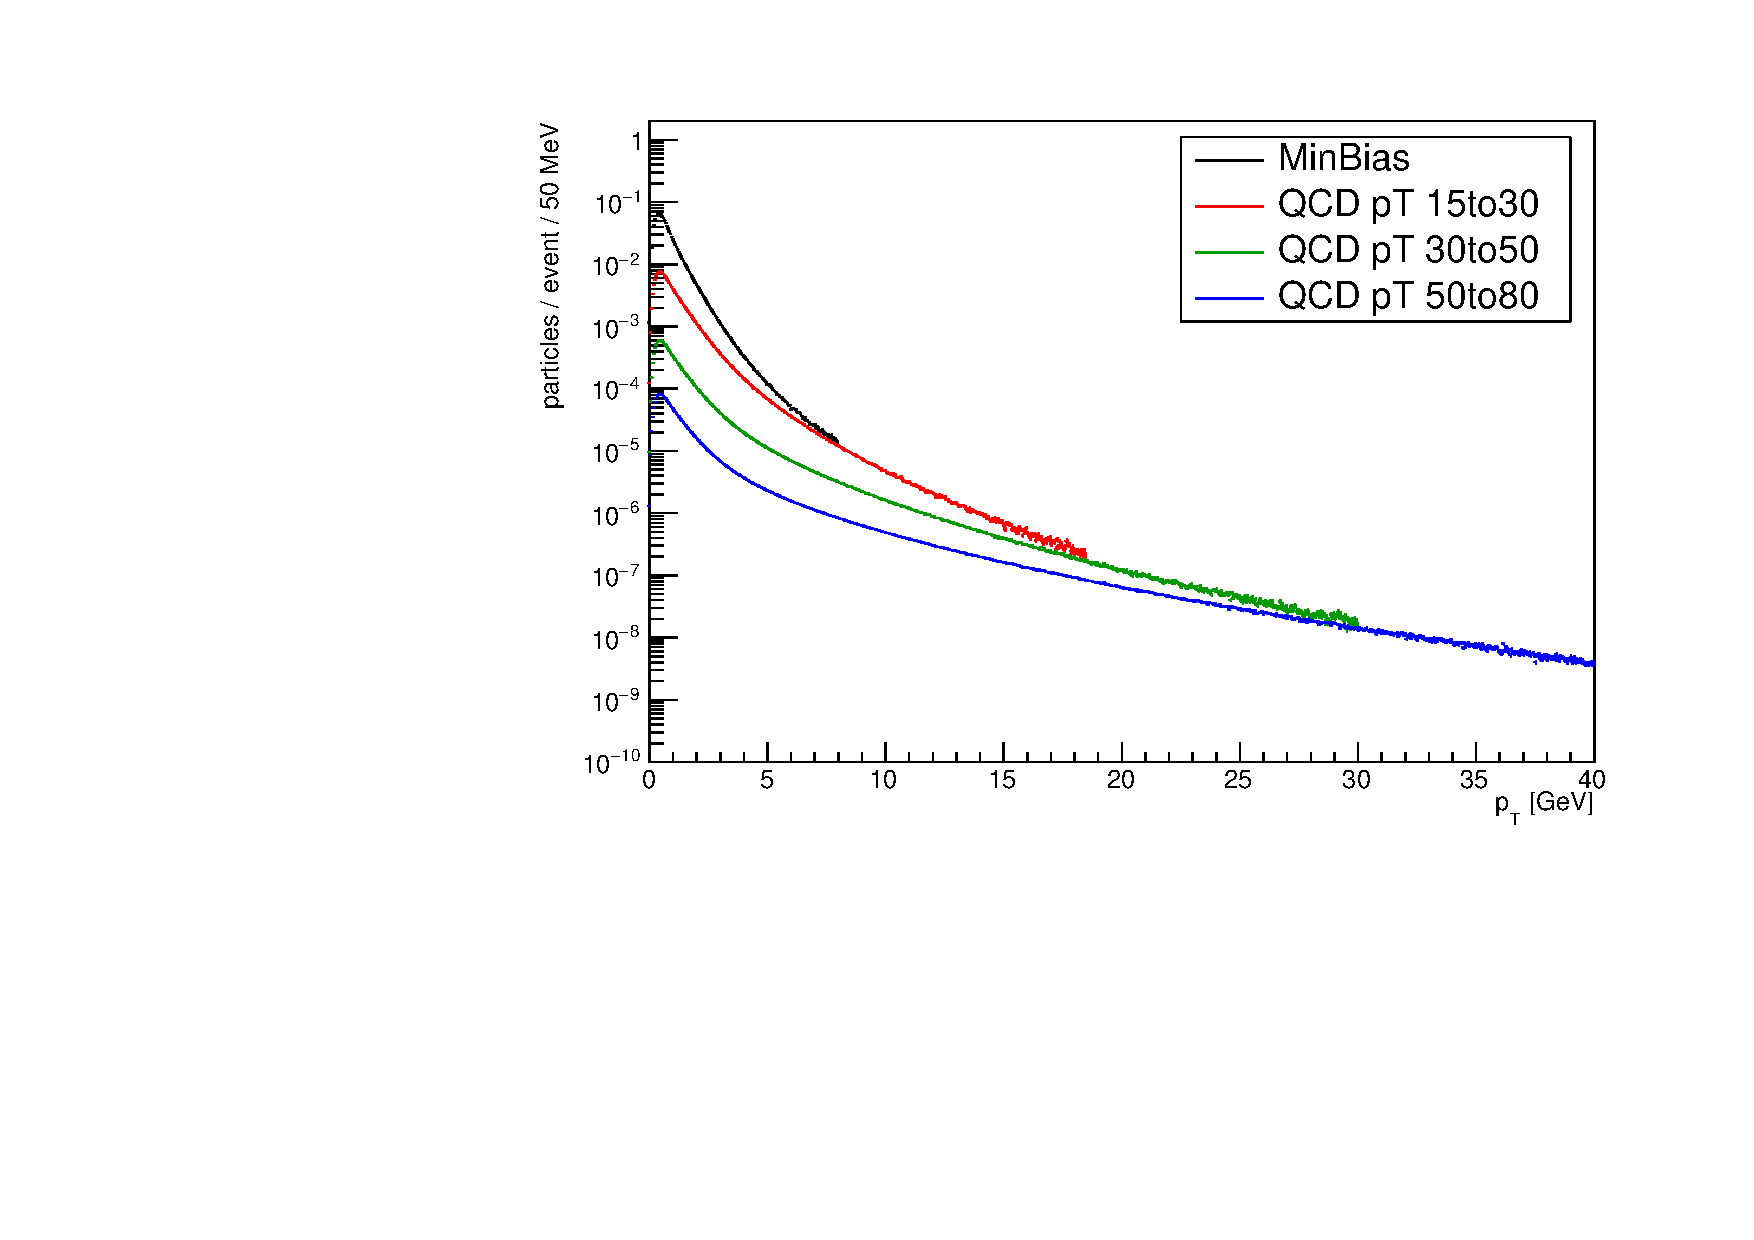
\includegraphics[width=0.48\linewidth]{plots/h_eta.pdf}
  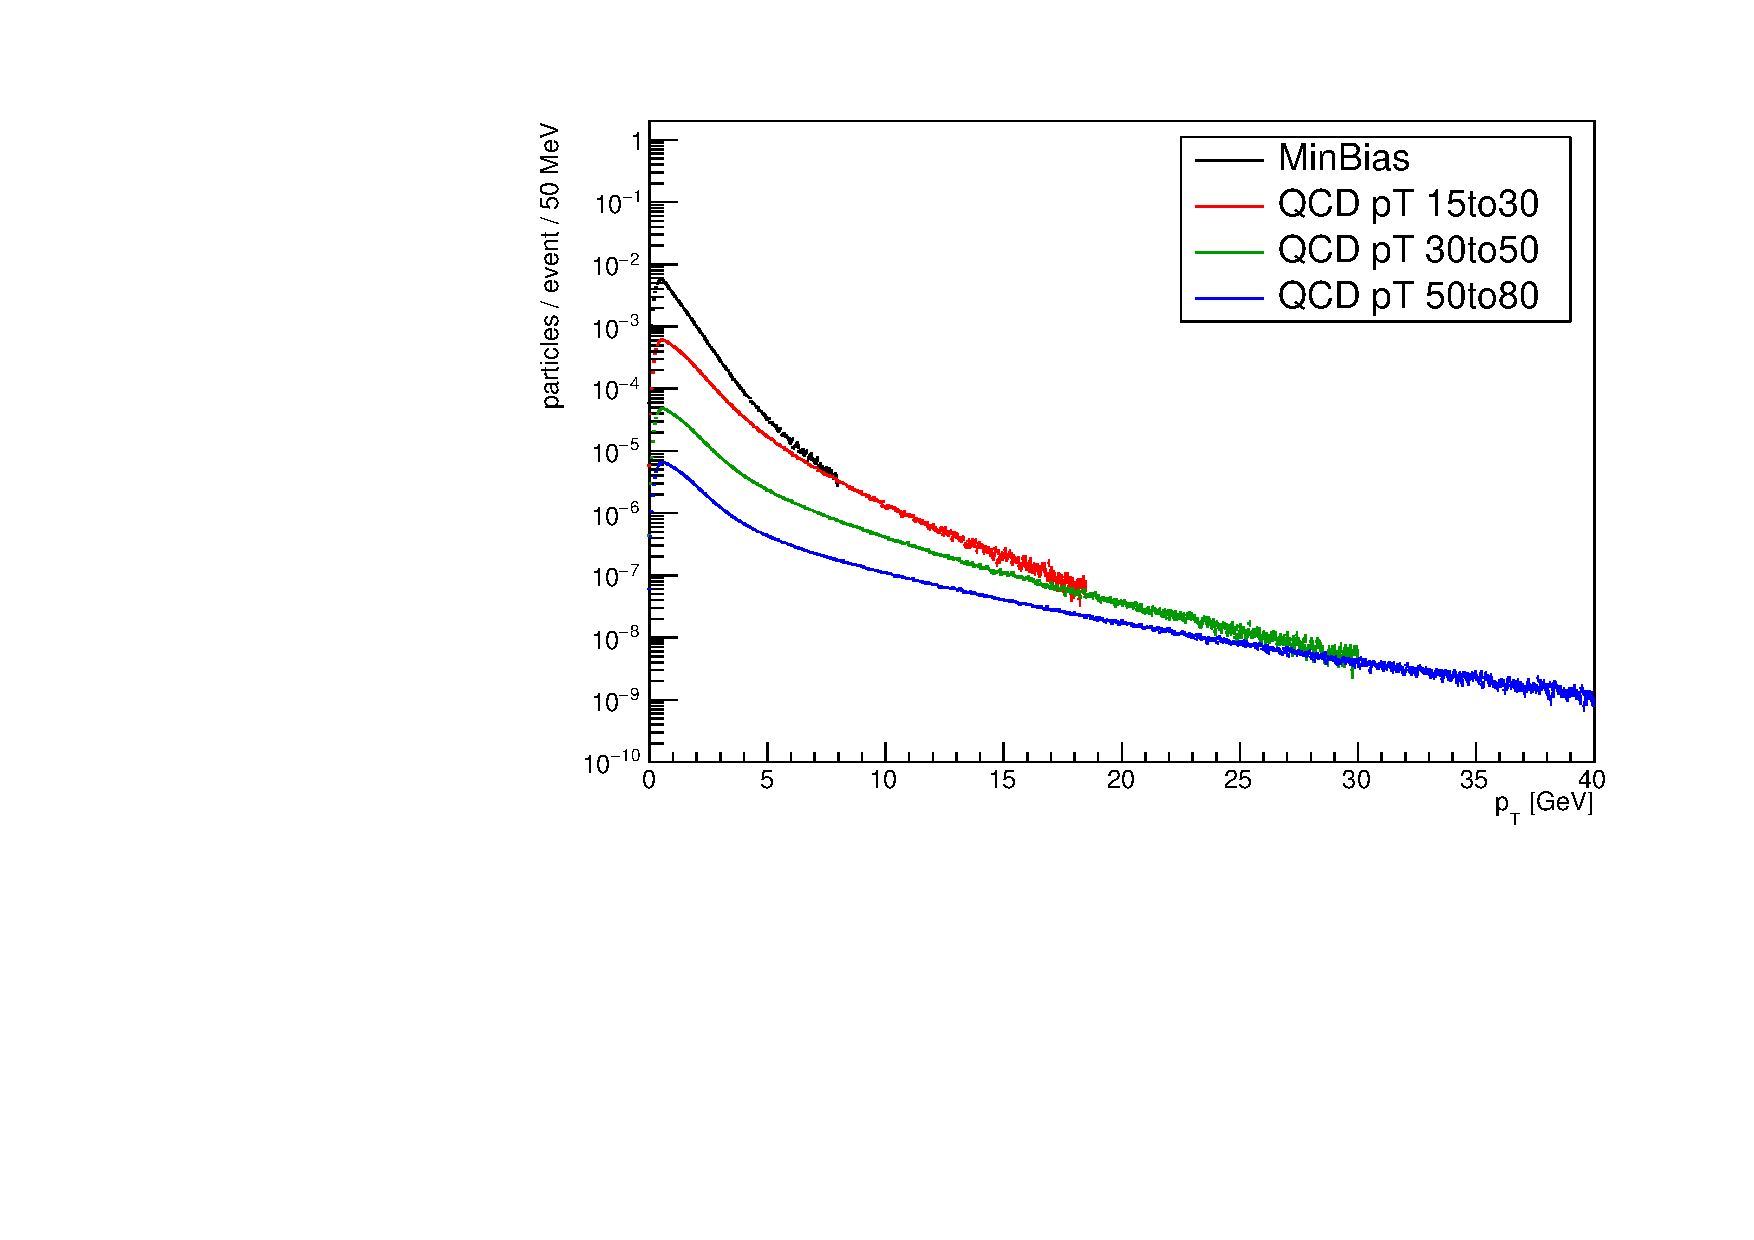
\includegraphics[width=0.48\linewidth]{plots/h_etap.pdf}
  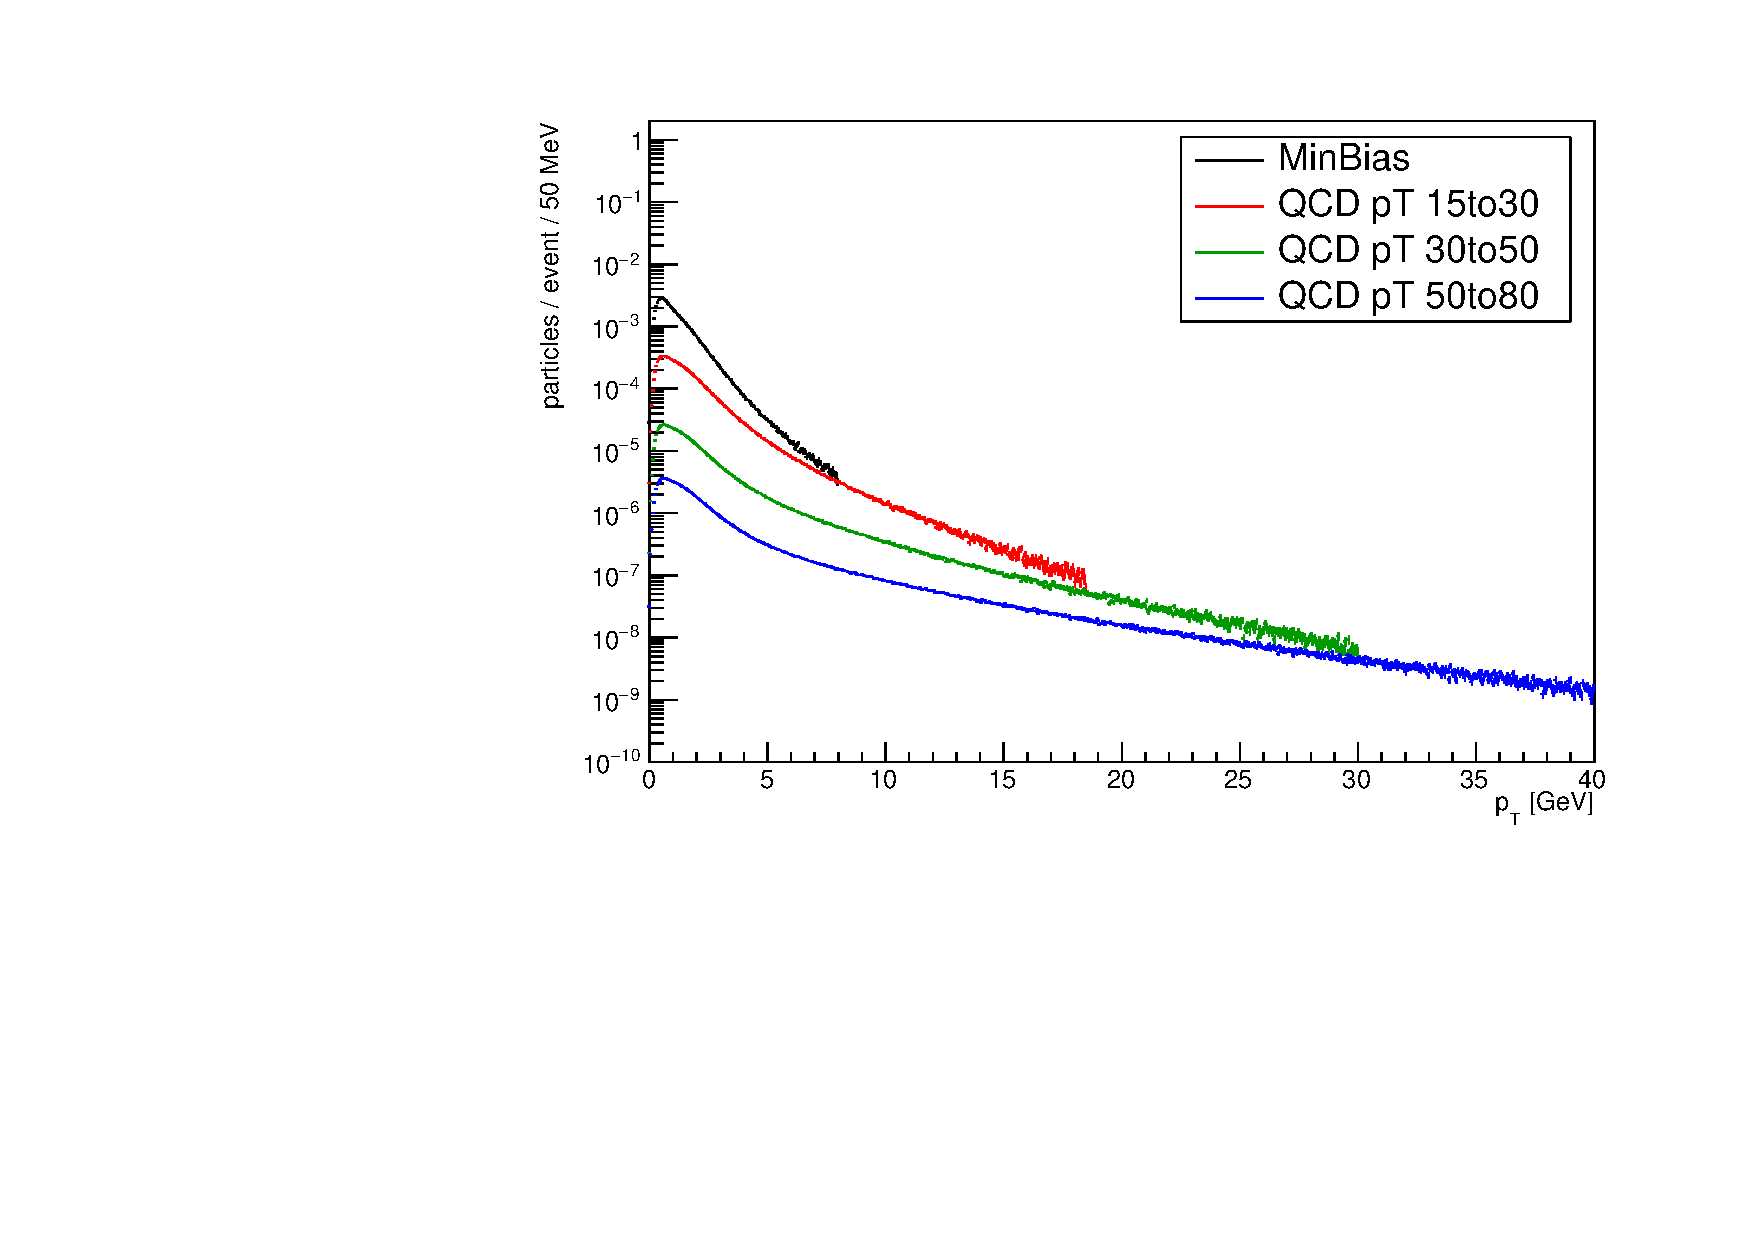
\includegraphics[width=0.48\linewidth]{plots/h_phi.pdf}
  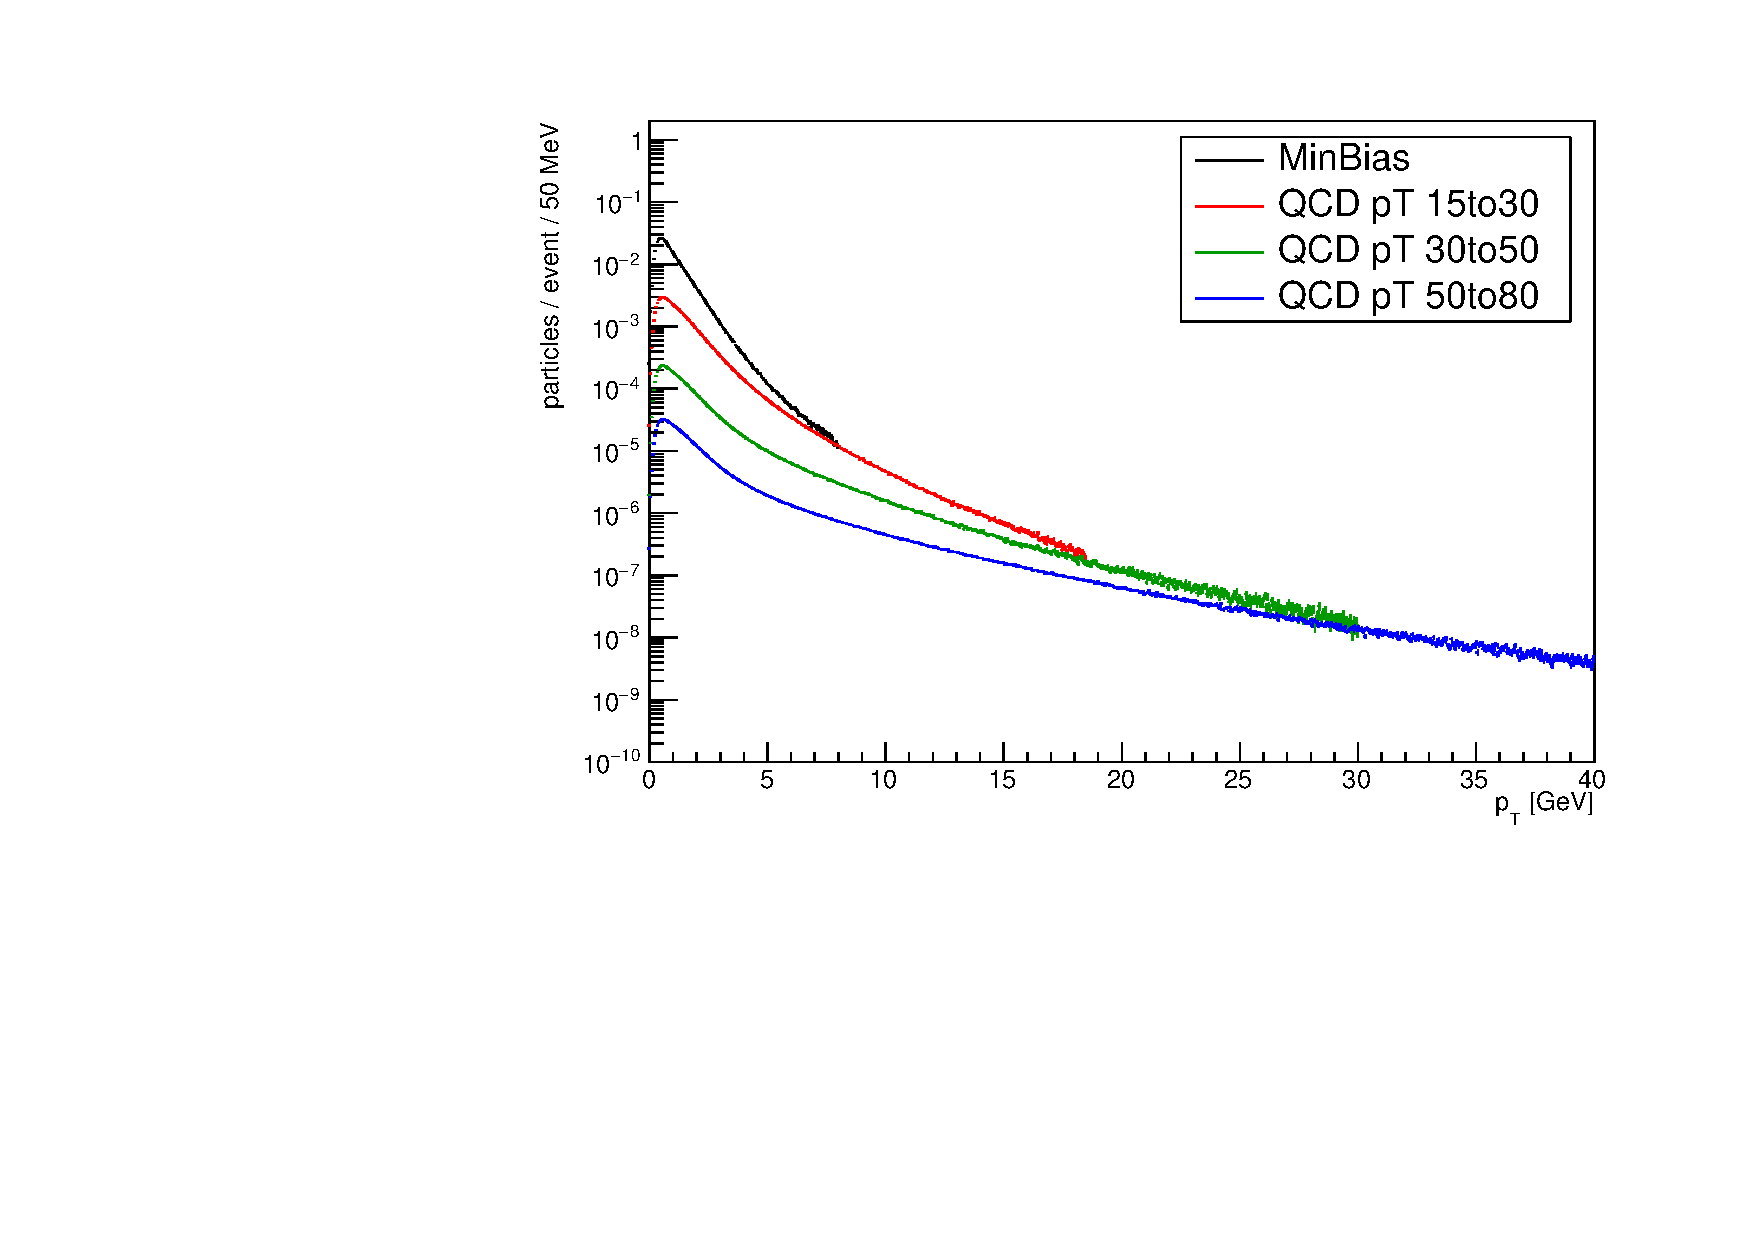
\includegraphics[width=0.48\linewidth]{plots/h_rho.pdf}
  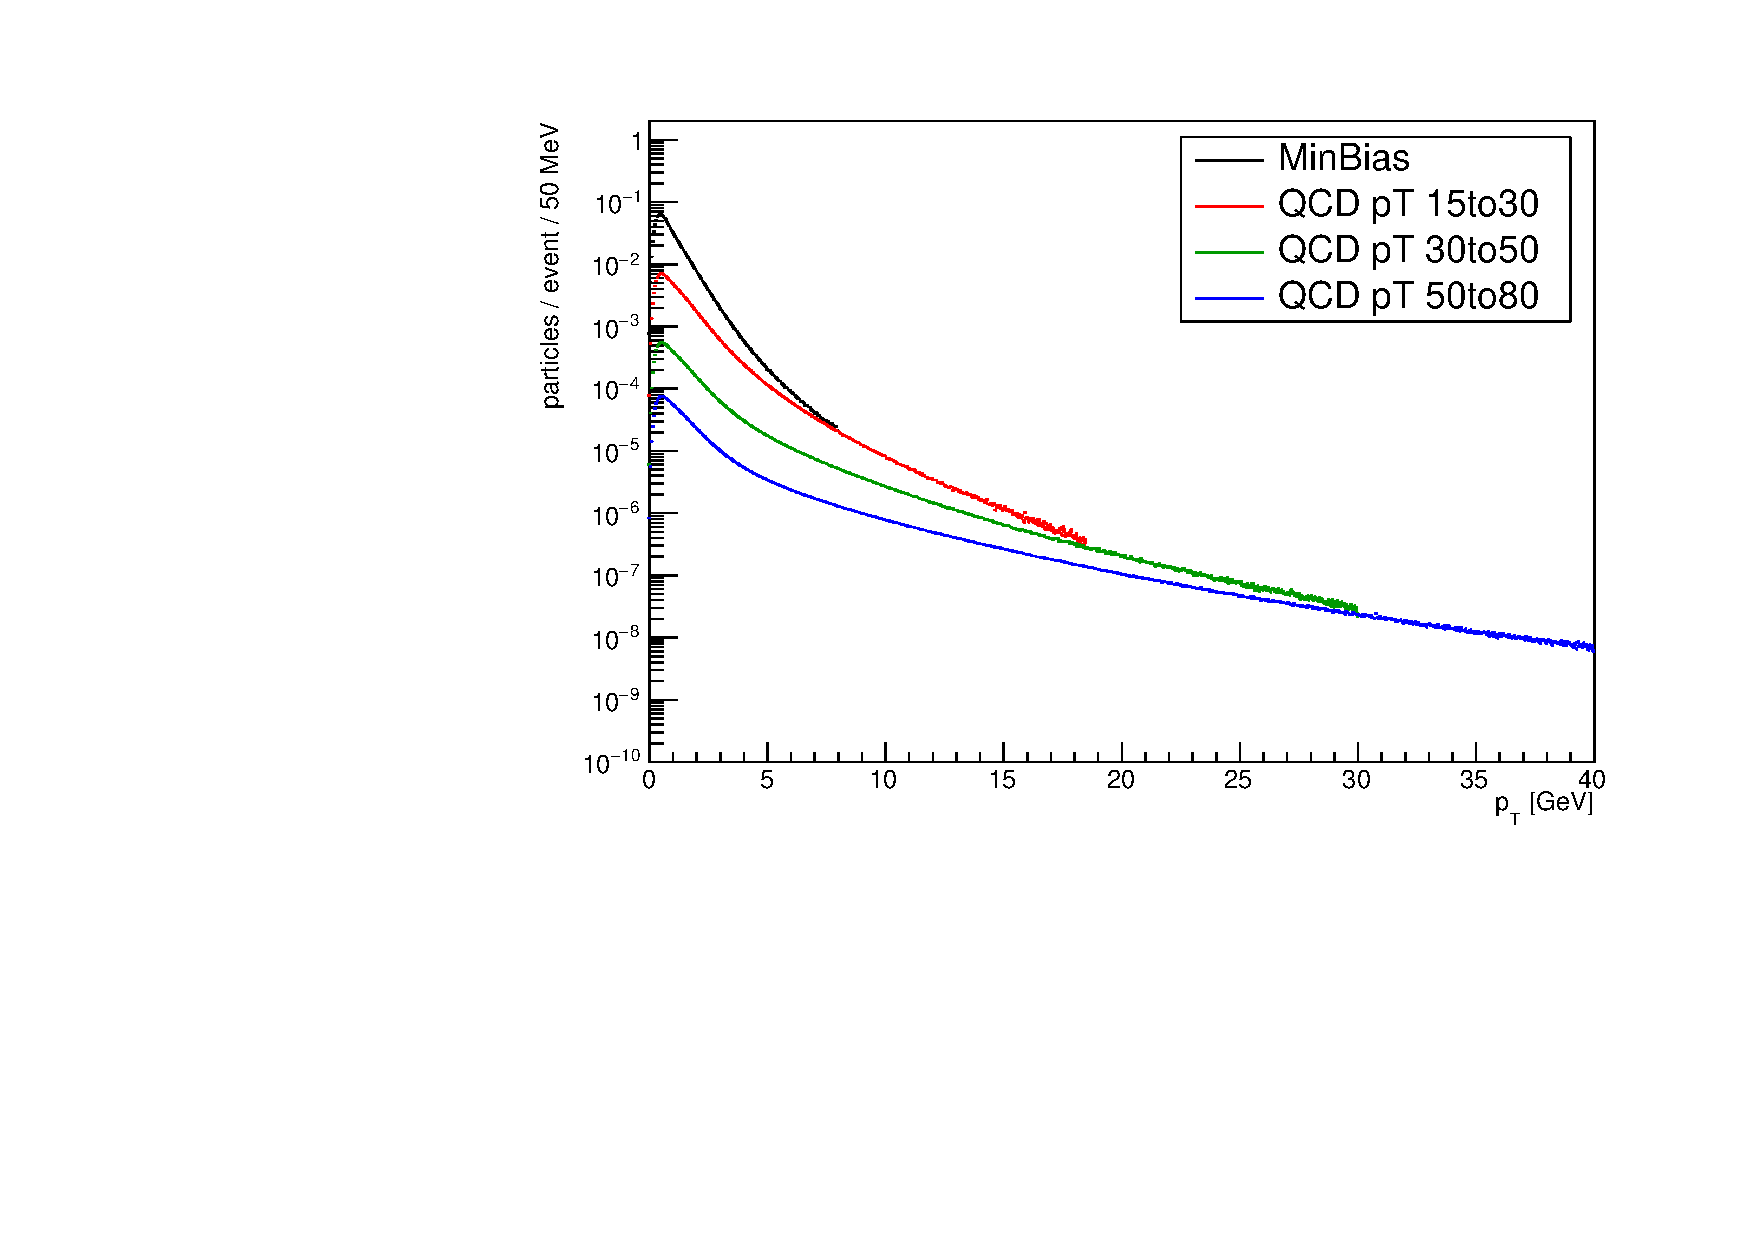
\includegraphics[width=0.48\linewidth]{plots/h_omega.pdf}
  \caption{\protect Transverse momentum distributions of 
$\pi^0$, $\eta$, $\eta'$, $\phi$, $\rho$, and $\omega$, top left
to bottom right, for $|\eta| < 1$.}
\label{fig:mesons}
\end{figure}


\clearpage
\begin{thebibliography}{1}

%\cite{Cacciari:2012ny,Cacciari:2015fta}
\bibitem{Cacciari:2012ny}
  M.~Cacciari, S.~Frixione, N.~Houdeau, M.~L.~Mangano, P.~Nason and G.~Ridolfi,
  % ``Theoretical predictions for charm and bottom
  % production at the LHC,''
  JHEP {\bf 1210} (2012) 137 [arXiv:1205.6344 [hep-ph]].
  %%CITATION = ARXIV:1205.6344;%%

\bibitem{Cacciari:2015fta}
  M.~Cacciari, M.~L.~Mangano and P.~Nason,
  %``Gluon PDF constraints from the ratio of forward heavy quark production at
  % the LHC at \sqrt{S}=7 and 13 TeV,''
  arXiv:1507.06197 [hep-ph].
  %%CITATION = ARXIV:1507.06197;%%

%\cite{Khachatryan:2010zg}
\bibitem{Khachatryan:2010zg} 
  V.~Khachatryan {\it et al.} [CMS Collaboration],
  %``Upsilon Production Cross-Section in pp Collisions at $sqrt{s}=7$ TeV,''
  Phys.\ Rev.\ D {\bf 83}, 112004 (2011)
  doi:10.1103/PhysRevD.83.112004
  [arXiv:1012.5545 [hep-ex]].
  %%CITATION = doi:10.1103/PhysRevD.83.112004;%%
  %143 citations counted in INSPIRE as of 22 Jun 2019

  %\cite{Chatrchyan:2013yna}
\bibitem{Chatrchyan:2013yna} 
  S.~Chatrchyan {\it et al.} [CMS Collaboration],
  %``Measurement of the $\Upsilon(1S), \Upsilon(2S)$, and $\Upsilon(3S)$ Cross Sections in $pp$ Collisions at $\sqrt{s}$ = 7 TeV,''
  Phys.\ Lett.\ B {\bf 727}, 101 (2013)
  doi:10.1016/j.physletb.2013.10.033
  [arXiv:1303.5900 [hep-ex]].
  %%CITATION = doi:10.1016/j.physletb.2013.10.033;%%
  %85 citations counted in INSPIRE as of 22 Jun 2019

%\cite{Khachatryan:2015qpa}
\bibitem{Khachatryan:2015qpa} 
  V.~Khachatryan {\it et al.} [CMS Collaboration],
  %``Measurements of the $\Upsilon$(1S), $\Upsilon$(2S), and $\Upsilon$(3S) differential cross sections in pp collisions at $\sqrt{s} =$ 7 TeV,''
  Phys.\ Lett.\ B {\bf 749}, 14 (2015)
  doi:10.1016/j.physletb.2015.07.037
  [arXiv:1501.07750 [hep-ex]].
  %%CITATION = doi:10.1016/j.physletb.2015.07.037;%%
  %36 citations counted in INSPIRE as of 22 Jun 2019


  %\cite{Sirunyan:2017qdw}
\bibitem{Sirunyan:2017qdw} 
  A.~M.~Sirunyan {\it et al.} [CMS Collaboration],
  %``Measurement of quarkonium production cross sections in pp collisions at $\sqrt{s}=$ 13 TeV,''
  Phys.\ Lett.\ B {\bf 780}, 251 (2018)
  doi:10.1016/j.physletb.2018.02.033
  [arXiv:1710.11002 [hep-ex]].
  %%CITATION = doi:10.1016/j.physletb.2018.02.033;%%
  %19 citations counted in INSPIRE as of 22 Jun 2019


  %\cite{Aad:2011xv}
\bibitem{Aad:2011xv}
  G.~Aad {\it et al.} [ATLAS Collaboration],
  %``Measurement of the $\Upsilon$(1S) production cross-section in $pp$ collisions at $\sqrt{s}=$ 7 TeV in ATLAS,''
  Phys.\ Lett.\ B {\bf 705} (2011) 9
  doi:10.1016/j.physletb.2011.09.092
  [arXiv:1106.5325 [hep-ex]].
  %%CITATION = doi:10.1016/j.physletb.2011.09.092;%%
  %44 citations counted in INSPIRE as of 22 Jun 2019

%\cite{Aad:2012dlq}
\bibitem{Aad:2012dlq} 
  G.~Aad {\it et al.} [ATLAS Collaboration],
  %``Measurement of Upsilon production in 7 TeV pp collisions at ATLAS,''
  Phys.\ Rev.\ D {\bf 87}, no. 5, 052004 (2013)
  doi:10.1103/PhysRevD.87.052004
  [arXiv:1211.7255 [hep-ex]].
  %%CITATION = doi:10.1103/PhysRevD.87.052004;%%
  %127 citations counted in INSPIRE as of 22 Jun 2019


%\cite{Aaij:2018pfp}
\bibitem{Aaij:2018pfp}
  R.~Aaij {\it et al.} [LHCb Collaboration],
  %``Measurement of $\Upsilon$ production in $pp$ collisions at $\sqrt{s}$= 13 TeV,''
  JHEP {\bf 1807} (2018) 134
   Erratum: [JHEP {\bf 1905} (2019) 076]
  doi:10.1007/JHEP07(2018)134, 10.1007/JHEP05(2019)076
  [arXiv:1804.09214 [hep-ex]].
  %%CITATION = doi:10.1007/JHEP07(2018)134, 10.1007/JHEP05(2019)076;%%
  %5 citations counted in INSPIRE as of 22 Jun 2019
  
  %\cite{Aaij:2015awa}
\bibitem{Aaij:2015awa}
  R.~Aaij {\it et al.} [LHCb Collaboration],
  %``Forward production of $\Upsilon$ mesons in $pp$ collisions at $\sqrt{s}=7$ and 8TeV,''
  JHEP {\bf 1511} (2015) 103
  doi:10.1007/JHEP11(2015)103
  [arXiv:1509.02372 [hep-ex]].
  %%CITATION = doi:10.1007/JHEP11(2015)103;%%
  %41 citations counted in INSPIRE as of 22 Jun 2019

  %\cite{Aaij:2014nwa}
\bibitem{Aaij:2014nwa}
  R.~Aaij {\it et al.} [LHCb Collaboration],
  %``Measurement of $\Upsilon$ production in $pp$ collisions at $\sqrt{s}=2.76$ TeV,''
  Eur.\ Phys.\ J.\ C {\bf 74} (2014) no.4,  2835
  doi:10.1140/epjc/s10052-014-2835-1
  [arXiv:1402.2539 [hep-ex]].
  %%CITATION = doi:10.1140/epjc/s10052-014-2835-1;%%
  %42 citations counted in INSPIRE as of 22 Jun 2019

  %\cite{Aaij:2013yaa}
\bibitem{Aaij:2013yaa} 
  R.~Aaij {\it et al.} [LHCb Collaboration],
  %``Production of J/psi and Upsilon mesons in pp collisions at sqrt(s) = 8 TeV,''
  JHEP {\bf 1306}, 064 (2013)
  doi:10.1007/JHEP06(2013)064
  [arXiv:1304.6977 [hep-ex]].
  %%CITATION = doi:10.1007/JHEP06(2013)064;%%
  %120 citations counted in INSPIRE as of 22 Jun 2019

%\cite{LHCb:2012aa}
\bibitem{LHCb:2012aa} 
  R.~Aaij {\it et al.} [LHCb Collaboration],
  %``Measurement of Upsilon production in pp collisions at $\sqrt{s}$ = 7 TeV,''
  Eur.\ Phys.\ J.\ C {\bf 72}, 2025 (2012)
  doi:10.1140/epjc/s10052-012-2025-y
  [arXiv:1202.6579 [hep-ex]].
  %%CITATION = doi:10.1140/epjc/s10052-012-2025-y;%%
  %127 citations counted in INSPIRE as of 22 Jun 2019

%\cite{Han:2014kxa}
\bibitem{Han:2014kxa} 
  H.~Han, Y.~Q.~Ma, C.~Meng, H.~S.~Shao, Y.~J.~Zhang and K.~T.~Chao,
  %``$\Upsilon(nS)$ and $\chi_b(nP)$ production at hadron colliders in nonrelativistic QCD,''
  Phys.\ Rev.\ D {\bf 94}, no. 1, 014028 (2016)
  doi:10.1103/PhysRevD.94.014028
  [arXiv:1410.8537 [hep-ph]].
  %%CITATION = doi:10.1103/PhysRevD.94.014028;%%
  %30 citations counted in INSPIRE as of 22 Jun 2019

  
\bibitem{Sirunyan:2017zmn} 
  A.~M.~Sirunyan {\it et al.} [CMS Collaboration],
  %``Measurement of charged pion, kaon, and proton production in proton-proton collisions at $\sqrt{s}=13$ TeV,''
  Phys.\ Rev.\ D {\bf 96}, no. 11, 112003 (2017)
  doi:10.1103/PhysRevD.96.112003
  [arXiv:1706.10194 [hep-ex]].
  %%CITATION = doi:10.1103/PhysRevD.96.112003;%%
  %25 citations counted in INSPIRE as of 20 Jun 2019

  
  
\bibitem{wwwPythia}
\href{http://home.thep.lu.se/\~torbjorn/pythia81php/Welcome.php}
{http://home.thep.lu.se/\~torbjorn/pythia81php/Welcome.php}.  Click on 
{\tt QCD} on th eleft panel.

\end{thebibliography}  
\end{document}
